\documentclass[a4paper]{book}
\usepackage{a4wide}
\usepackage{makeidx}
\usepackage{fancyhdr}
\usepackage{graphicx}
\usepackage{multicol}
\usepackage{float}
\usepackage{textcomp}
\usepackage{alltt}
\usepackage[utf8]{inputenc}
\usepackage{doxygen}
\makeindex
\setcounter{tocdepth}{1}
\renewcommand{\footrulewidth}{0.4pt}
\begin{document}
\begin{titlepage}
\vspace*{7cm}
\begin{center}
{\Large QuaZIP \\[1ex]\large quazip-0-2-3 }\\
\vspace*{1cm}
{\large Generated by Doxygen 1.5.5}\\
\vspace*{0.5cm}
{\small Wed Sep 17 11:17:59 2008}\\
\end{center}
\end{titlepage}
\clearemptydoublepage
\pagenumbering{roman}
\tableofcontents
\clearemptydoublepage
\pagenumbering{arabic}
\chapter{QuaZIP - Qt/C++ wrapper for ZIP/UNZIP package }
\label{index} \section{Overview}\label{index_overview}
QuaZIP is a simple C++ wrapper over {\tt Gilles Vollant's ZIP/UNZIP package} that can be used to access ZIP archives. It uses {\tt Trolltech's Qt toolkit}.

If you do not know what Qt is, you have two options:\begin{itemize}
\item Just forget about QuaZIP.\item Learn more about Qt by downloading it and/or reading excellent {\tt official Qt documentation}\end{itemize}


The choice is yours, but if you are really interested in cross-platform (Windows/Linux/BSD/UNIX/Mac/Others) software development, I would definitely recommend you the second choice $^\wedge$\_\-$^\wedge$

QuaZIP allows you to access files inside ZIP archives using QIODevice API, and - yes! - that means that you can also use QTextStream, QDataStream or whatever you would like to use on your zipped files.

QuaZIP provides complete abstraction of the ZIP/UNZIP API, for both reading from and writing to ZIP archives.\section{Platforms supported}\label{index_platforms}
QuaZIP has been currently tested with Qt 4.0.0 on the following platforms:\begin{itemize}
\item linux-g++\item freebsd-g++\item hpux-acc\item win32-g++ (MinGW)\end{itemize}


No testing has been done on other systems. Of course, patches to make it work on any platform that it currently does not work on are always welcome!\section{What is new in this version of QuaZIP?}\label{index_whats-new}
See NEWS file supplied with the distribution.\section{Getting latest version of QuaZIP}\label{index_getting}
Check {\tt QuaZIP project's page at SourceForge.net}. Also, you may wish to read latest version documentation available at the {\tt QuaZIP web site}.\section{Requirements}\label{index_Requirements}
Just {\tt zlib} and Qt 4. Well, Qt 4 depends on zlib anyway.\section{Building, testing and installing}\label{index_building}
\begin{Desc}
\item[Note:]Instructions given in this section assume that you are using some UNIX dialect, but the build process should be very similar on win32-g++ platform too. Sorry, but other platforms are undocumented. I do not think it is a big deal, though - it is standard usage of the Qt's qmake, so you most probably already know everything that is required.\end{Desc}
To build it on some UNIX dialect: 

\footnotesize\begin{verbatim}
$ cd /wherever/quazip/source/is/quazip-x.y.z/quazip
$ qmake [PREFIX=where-to-install]
$ make
\end{verbatim}
\normalsize


Make sure that you have Qt 4 installed with all required headers and utilities (not just library) and that you run qmake utility of the Qt 4, not some other version you may have already installed (you may need to type full path to qmake like /usr/local/qt4/bin/qmake).

To reconfigure (with another PREFIX, for example), just run qmake with appropriate arguments again.

If you need to specify additional include path or libraries, use qmake features (see qmake reference in the Qt documentation). For example:



\footnotesize\begin{verbatim}
$ qmake LIBS+=-L/usr/local/zlib/lib INCLUDEPATH+=/usr/local/zlib/include
\end{verbatim}
\normalsize
 (note abscence of \char`\"{}-I\char`\"{} before include path)

To check if QuaZIP's basic features work ok on your platform, you may wish to compile simple test programs provided in test directory. Look in the sources of the tests to find out about their requirements. Typically, the test looks something like this: 

\footnotesize\begin{verbatim}
$ cd /wherever/quazip/source/is/quazip-x.y.z/test/zip
$ qmake
$ make
$ ./zip
$ cd ../unzip
$ cp ../zip/test.zip ./test.zip
$ mkdir out
$ qmake
$ make
$ ./unzip
\end{verbatim}
\normalsize


You should see the zip contents with details as the output of the \char`\"{}./unzip\char`\"{}. Ignore message saying you should check the file name for testCase() if you do not want to test \doxyref{locale-aware case-insensitivity}{p.}{classQuaZip_6053a1d249ed210a85c9d5eb7cf9cdbe}. Otherwise, see the sources. In any case, this message appearing means that everything else was fine. Otherwise, you will get some other error message instead. Investigate it or send bug report including message, platform and QuaZIP version used.

To install compiled library: 

\footnotesize\begin{verbatim}
$ make install
\end{verbatim}
\normalsize


By default, QuaZIP compiles as static library, but you have other options:\begin{itemize}
\item Just copy appropriate source files to your project and use them;\item Compile QuaZIP as shared library by changing \char`\"{}staticlib\char`\"{} in quazip/quazip.pro to \char`\"{}dll\char`\"{}.\end{itemize}


Latter is not recommended because future versions of QuaZIP most probably will be binary incompatible.\section{Using}\label{index_using}
See \doxyref{usage page}{p.}{usage}.\section{Bugs}\label{index_bugs}
QuaZIP is currently at the initial development stage. Therefore, there are may be plenty of bugs and other bad things. Bug reports and patches are always welcome (see \char`\"{}contacts\char`\"{} below).\section{Authors and contacts}\label{index_contacts}
This wrapper has been written by Sergey A. Tachenov, AKA Alqualos. This is my first open source project, so it may suck, but I did not find anything like that, so I just had no other choice but to write it.

If you have anything to say to me about QuaZIP library, feel free to do so (read the \doxyref{QuaZip FAQ}{p.}{faq} first, though). I can not promise, though, that I fix all the bugs you report in, add any features you want, or respond to your critics, or respond to your feedback at all. I may be busy, I may be tired of working on QuaZIP, I may be even dead already (you never know...). But regardless of this remark, any feedback is always welcome. This may seem like a paradox to you, but you do not have to understand it to write feedback.

To report bugs or to post ideas about what should be done, use SourceForge.net's {\tt trackers}. If you want to send me a private message, use my e-mail address laerel at yandex dot ru (but do not you dare to put it somewhere on the Web or wherever).

Do not use e-mail to report bugs, please. Reporting bugs and problems with the SourceForge.net's bug report system has that advantage that it is visible to public.\section{My other projects}\label{index_other-projects}
As of this moment, I did not write any other useful open source software (well, I am too lazy to do it) except for one little thing:

{\tt Arcanum universal cap remover}. Arcanum is the old but very good game, which has one stupid limit: your character maximum level is 50, which is too low for many players including me. So I wrote this simple patch to increase this stupid limit to something acceptable.

Also, my first Web project, which can be of any interest to you only if you can read Russian and you are crazy $^\wedge$\_\-- This is a web site with the main topic of it being The Delirium. It is totally meaningless and it was purposely made to be such. Do not ask me why - I do not know either. I just did that. If you are interested, then welcome to {\tt The Brededor}. It does not get updated lately because I have become even lazier than I ever was. But I do not plan to destroy The Brededor no matter what, because I think it is fun.

Copyright (C) 2005-2007 Sergey A. Tachenov 
\chapter{QuaZip FAQ}
\label{faq_faq-GPL}
 Q. Is it possible to release an LGPL version of the \doxyref{QuaZip}{p.}{classQuaZip}?

A. I do not know much about licensing, so I can answer for sure, but \doxyref{QuaZip}{p.}{classQuaZip} was developed using Open Source edition of Qt, so I see no way it could be released under anything except GPL.

\label{faq_faq-non-QIODevice}
 Q. Is there any way to use \doxyref{QuaZipFile}{p.}{classQuaZipFile} in Qt where you are supposed to use normal (non-zipped) file, but not through QIODevice API?

A. Usually not. For example, if you are passing file name to some database driver (like SQLite), Qt usually just passes this name down to the 3rd-party library, which is usually does not know anything about QIODevice and therefore there is no way to pass \doxyref{QuaZipFile}{p.}{classQuaZipFile} as normal file. However, if we are talking about some place where you pass file name, and then indirectly use QFile to open it, then it is a good idea to make overloaded method, which accepts QIODevice pointer. Then you would be able to pass \doxyref{QuaZipFile}{p.}{classQuaZipFile} as well as many other nice things such as QBuffer or QProcess. 
\chapter{Usage}
This page provides general information on QuaZIP usage. See classes \doxyref{QuaZip}{p.}{classQuaZip} and \doxyref{QuaZipFile}{p.}{classQuaZipFile} for the detailed documentation on what can QuaZIP do and what can not. Also, reading comments in the zip.h and unzip.h files (taken from the original ZIP/UNZIP package) is always a good idea too. After all, QuaZIP is just a wrapper with a few convenience extensions and reimplementations.

\doxyref{QuaZip}{p.}{classQuaZip} is a class representing ZIP archive, \doxyref{QuaZipFile}{p.}{classQuaZipFile} represents a file inside archive and subclasses QIODevice as well.\section{Terminology}\label{usage_terminology}
\char`\"{}QuaZIP\char`\"{} means whole this library, while \char`\"{}QuaZip\char`\"{} (not case difference) is just one class in it.

\char`\"{}ZIP/UNZIP API\char`\"{} means the original API of the Gilles Vollant's ZIP/UNZIP package. I did not alter it in any way to make it easier to port to the future ZIP/UNZIP versions.

\char`\"{}ZIP\char`\"{}, \char`\"{}ZIP archive\char`\"{} or \char`\"{}ZIP file\char`\"{} means any ZIP archive. Typically this is a plain file with \char`\"{}.zip\char`\"{} (or \char`\"{}.ZIP\char`\"{}) file name suffix.

\char`\"{}A file inside archive\char`\"{}, \char`\"{}a file inside ZIP\char`\"{} or something like that means file either being read or written from/to some ZIP archive.\section{Error handling}\label{usage_error-handling}
Almost any call to ZIP/UNZIP API return some error code. Most of the original API's error checking could be done in this wrapper as well, but it would cause unnecessary code bloating without any benefit. So, QuaZIP only checks for situations that ZIP/UNZIP API can not check for. For example, ZIP/UNZIP API has no \char`\"{}ZIP open mode\char`\"{} concept because read and write modes are completely separated. On the other hand, to avoid creating classes like \char`\"{}QuaZipReader\char`\"{}, \char`\"{}QuaZipWriter\char`\"{} or something like that, QuaZIP introduces \char`\"{}ZIP open mode\char`\"{} concept instead, thus making it possible to use one class (\doxyref{QuaZip}{p.}{classQuaZip}) for both reading and writing. But this leads to additional open mode checks which are not done in ZIP/UNZIP package.

Therefore, error checking is two-level (QuaZIP's level and ZIP/UNZIP API level), which sometimes can be confusing, so here are some advices on how the error checking should be properly done:

\begin{itemize}
\item Both \doxyref{QuaZip}{p.}{classQuaZip} and \doxyref{QuaZipFile}{p.}{classQuaZipFile} have getZipError() function, which return error code of the last ZIP/UNZIP API call. Most function calls reset error code to UNZ\_\-OK on success and set error code on failure. Some functions do not reset error code. Most of them are {\tt const} and do not access ZIP archive in any way. Some, on the other hand, {\em do\/} access ZIP archive, but do not reset or set error code. For example, \doxyref{QuaZipFile::pos()}{p.}{classQuaZipFile_90fd55dab83eca7f95df50b2c41b7f22} function. Such functions are explicitly marked in the documentation.\item Most functions have its own way to report errors, by returning a null string, negative value or {\tt false}. If such a function returns error value, call getZipError() to get more information about error. See \char`\"{}zip.h\char`\"{} and \char`\"{}unzip.h\char`\"{} of the ZIP/UNZIP package for error codes.\item If the function returns error-stating value (like {\tt false}), but getZipError() returns UNZ\_\-OK, it means that you did something obviously wrong. For example, tried to write in the archive open for reading or not open at all. You better just do not do that! Most functions also issue a warning using qWarning() function in such cases. See documentation for a specific function for details on when it should not be called.\end{itemize}


I know that this is somewhat messy, but I could not find a better way to do all the error handling. 
\chapter{Directory Hierarchy}
\section{Directories}
This directory hierarchy is sorted roughly, but not completely, alphabetically:\begin{CompactList}
\item \contentsline{section}{quazip}{\pageref{dir_d5f2bee049160df10aa2fd550557f61f}}{}
\item \contentsline{section}{test}{\pageref{dir_d72eaf431c8ab2446754c0091103dfa0}}{}
\begin{CompactList}
\item \contentsline{section}{unzip}{\pageref{dir_0d290f915246044ba3a14f034cd1d91c}}{}
\begin{CompactList}
\item \contentsline{section}{out}{\pageref{dir_19179835fd1322ffa7e558f0c650ee3a}}{}
\end{CompactList}
\item \contentsline{section}{zip}{\pageref{dir_ee4c44d0388c12031fb738965cf777e7}}{}
\end{CompactList}
\end{CompactList}

\chapter{Class Index}
\section{Class List}
Here are the classes, structs, unions and interfaces with brief descriptions:\begin{CompactList}
\item\contentsline{section}{{\bf QuaZip} (ZIP archive )}{\pageref{classQuaZip}}{}
\item\contentsline{section}{{\bf QuaZipFile} (A file inside ZIP archive )}{\pageref{classQuaZipFile}}{}
\item\contentsline{section}{{\bf QuaZipFileInfo} (Information about a file inside archive )}{\pageref{structQuaZipFileInfo}}{}
\item\contentsline{section}{{\bf QuaZipNewInfo} (Information about a file to be created )}{\pageref{structQuaZipNewInfo}}{}
\end{CompactList}

\chapter{Directory Documentation}
\section{test/unzip/out/ Directory Reference}
\label{dir_19179835fd1322ffa7e558f0c650ee3a}\index{test/unzip/out/ Directory Reference@{test/unzip/out/ Directory Reference}}


\nopagebreak
\begin{figure}[H]
\begin{center}
\leavevmode
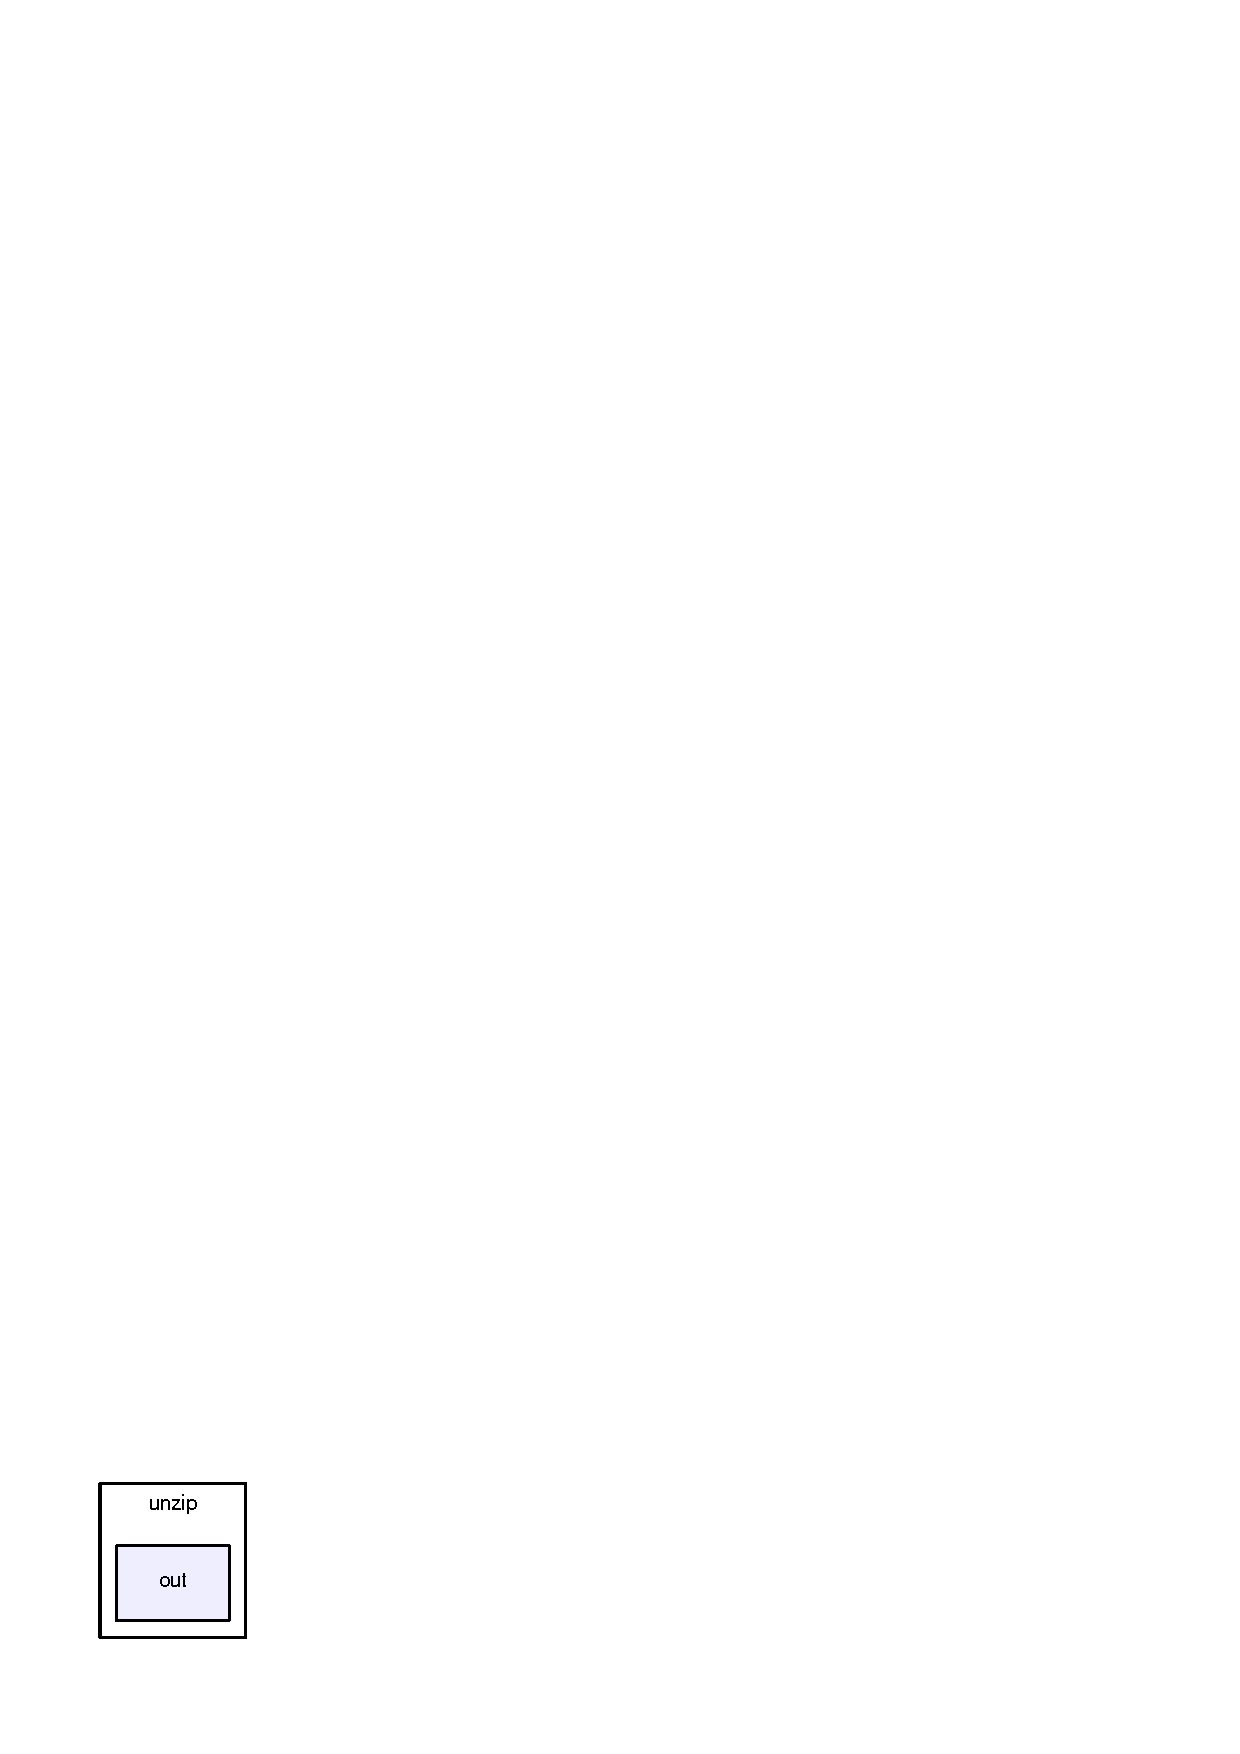
\includegraphics[width=65pt]{dir_19179835fd1322ffa7e558f0c650ee3a_dep}
\end{center}
\end{figure}
\subsection*{Files}
\begin{CompactItemize}
\item 
file \textbf{main.cpp}
\end{CompactItemize}

\section{quazip/ Directory Reference}
\label{dir_d5f2bee049160df10aa2fd550557f61f}\index{quazip/ Directory Reference@{quazip/ Directory Reference}}


\nopagebreak
\begin{figure}[H]
\begin{center}
\leavevmode
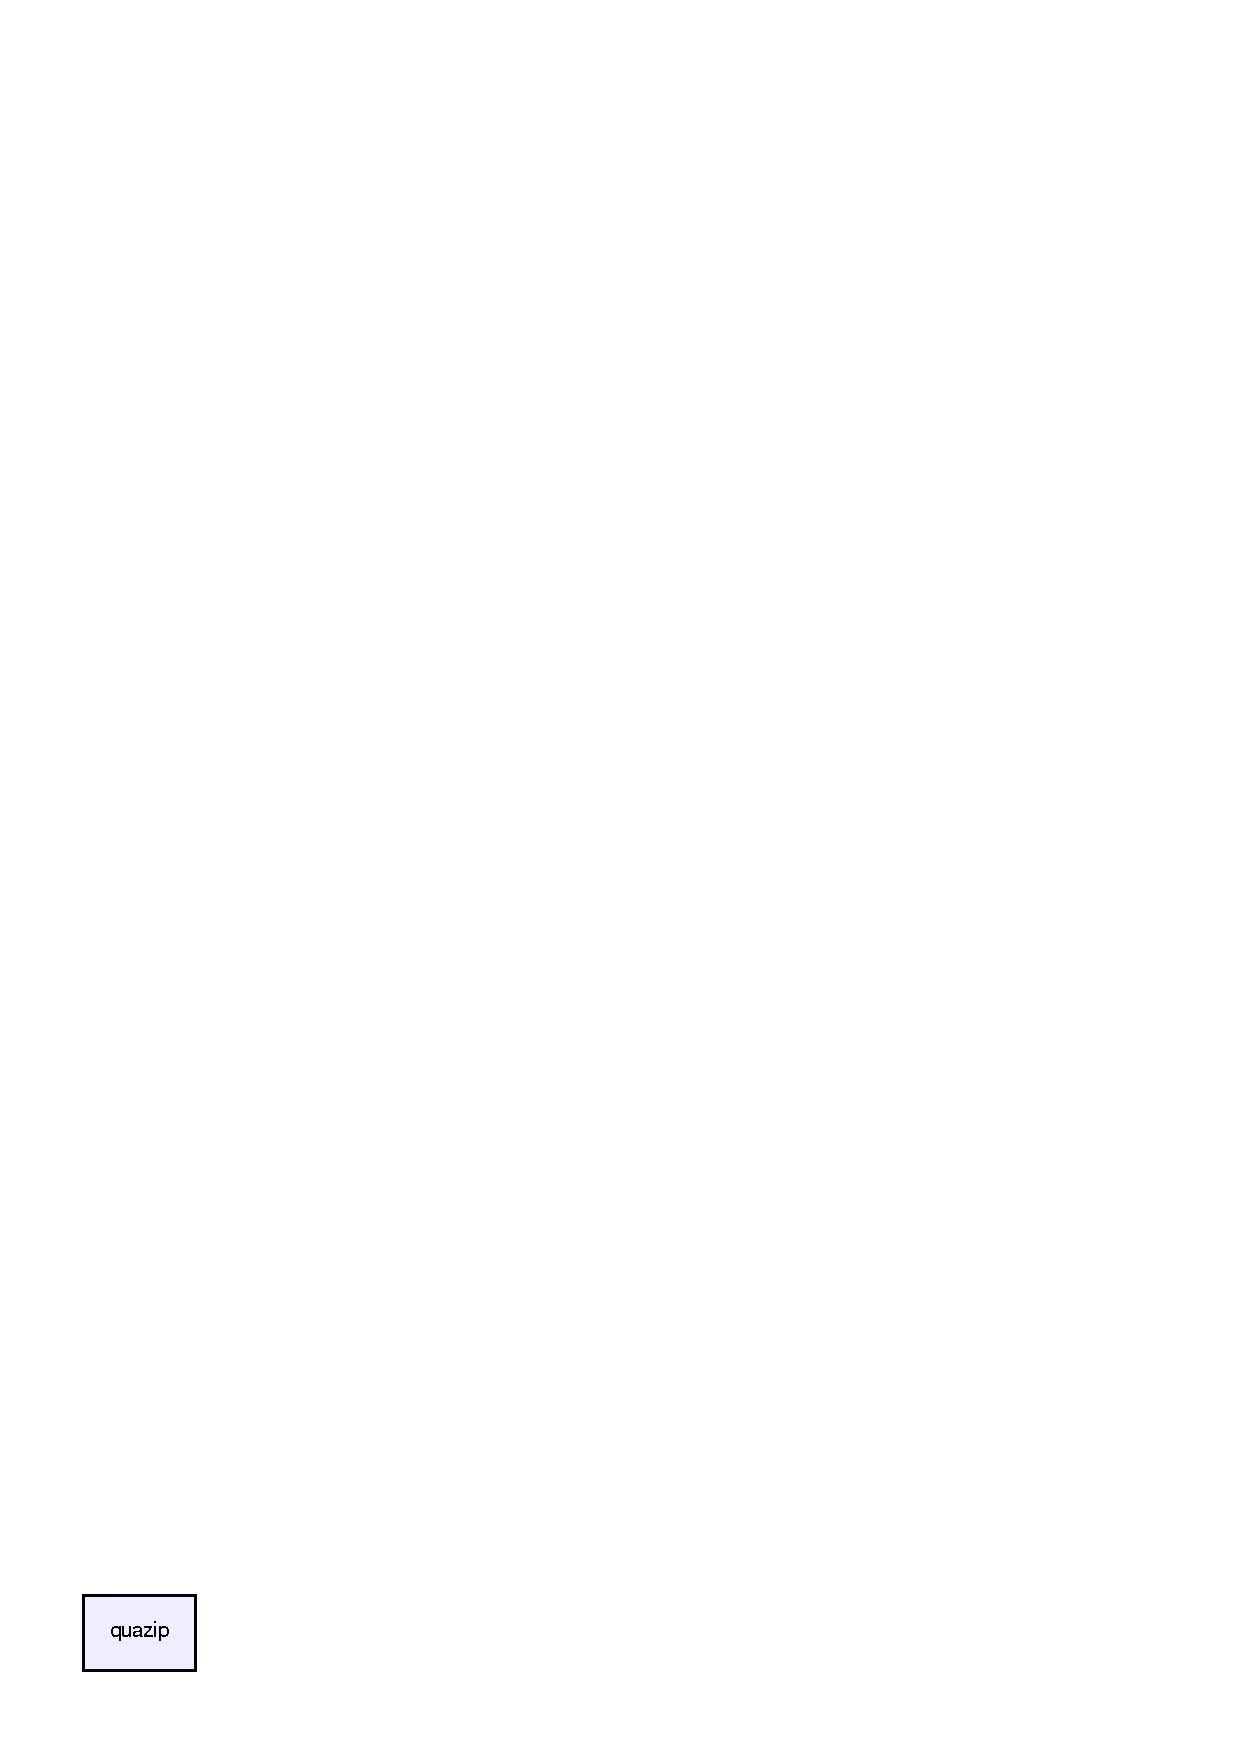
\includegraphics[width=49pt]{dir_d5f2bee049160df10aa2fd550557f61f_dep}
\end{center}
\end{figure}
\subsection*{Files}
\begin{CompactItemize}
\item 
file \textbf{quazip.cpp}
\item 
file \textbf{quazip.h}
\item 
file \textbf{quazipfile.cpp}
\item 
file \textbf{quazipfile.h}
\item 
file \textbf{quazipfileinfo.h}
\item 
file \textbf{quazipnewinfo.cpp}
\item 
file \textbf{quazipnewinfo.h}
\end{CompactItemize}

\section{test/ Directory Reference}
\label{dir_d72eaf431c8ab2446754c0091103dfa0}\index{test/ Directory Reference@{test/ Directory Reference}}


\nopagebreak
\begin{figure}[H]
\begin{center}
\leavevmode
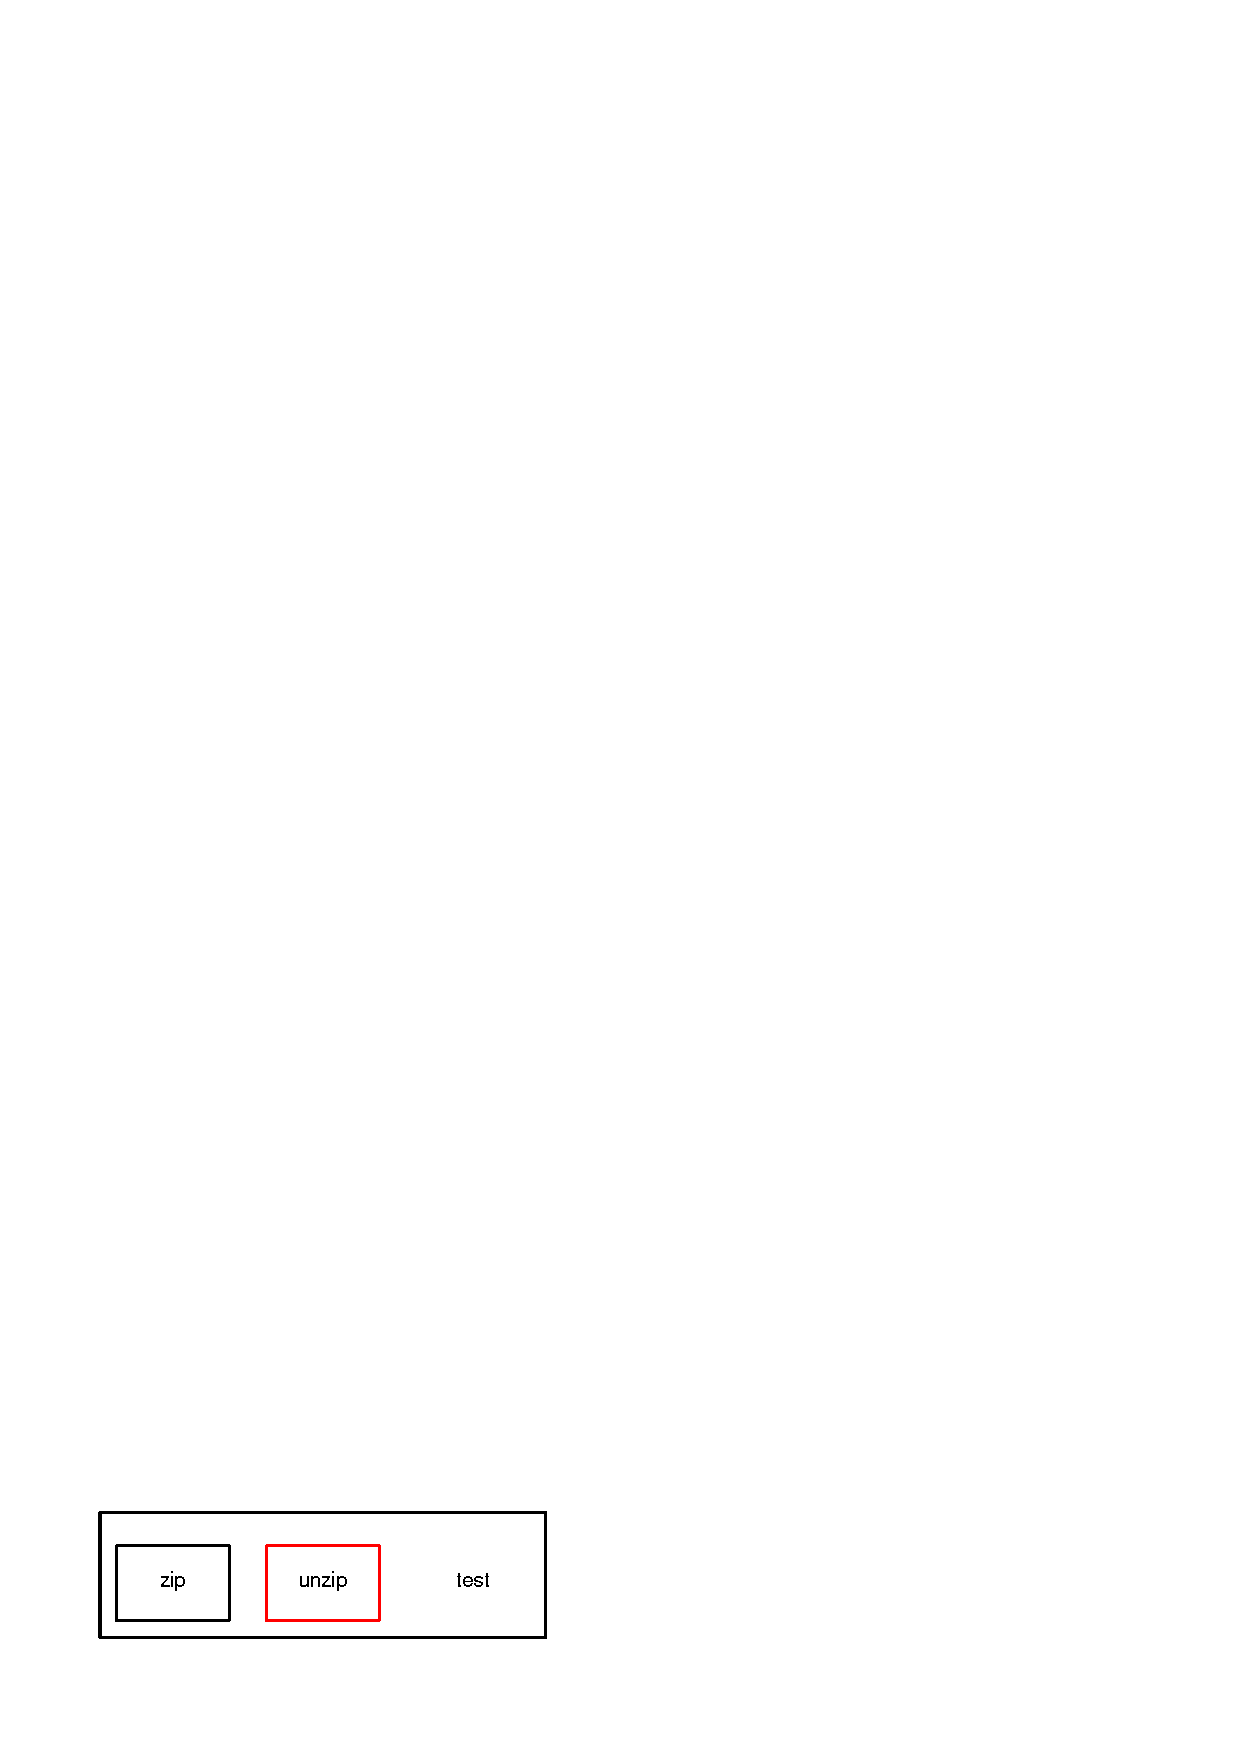
\includegraphics[width=137pt]{dir_d72eaf431c8ab2446754c0091103dfa0_dep}
\end{center}
\end{figure}
\subsection*{Directories}
\begin{CompactItemize}
\item 
directory {\bf unzip}
\item 
directory {\bf zip}
\end{CompactItemize}

\section{test/unzip/ Directory Reference}
\label{dir_0d290f915246044ba3a14f034cd1d91c}\index{test/unzip/ Directory Reference@{test/unzip/ Directory Reference}}


\nopagebreak
\begin{figure}[H]
\begin{center}
\leavevmode
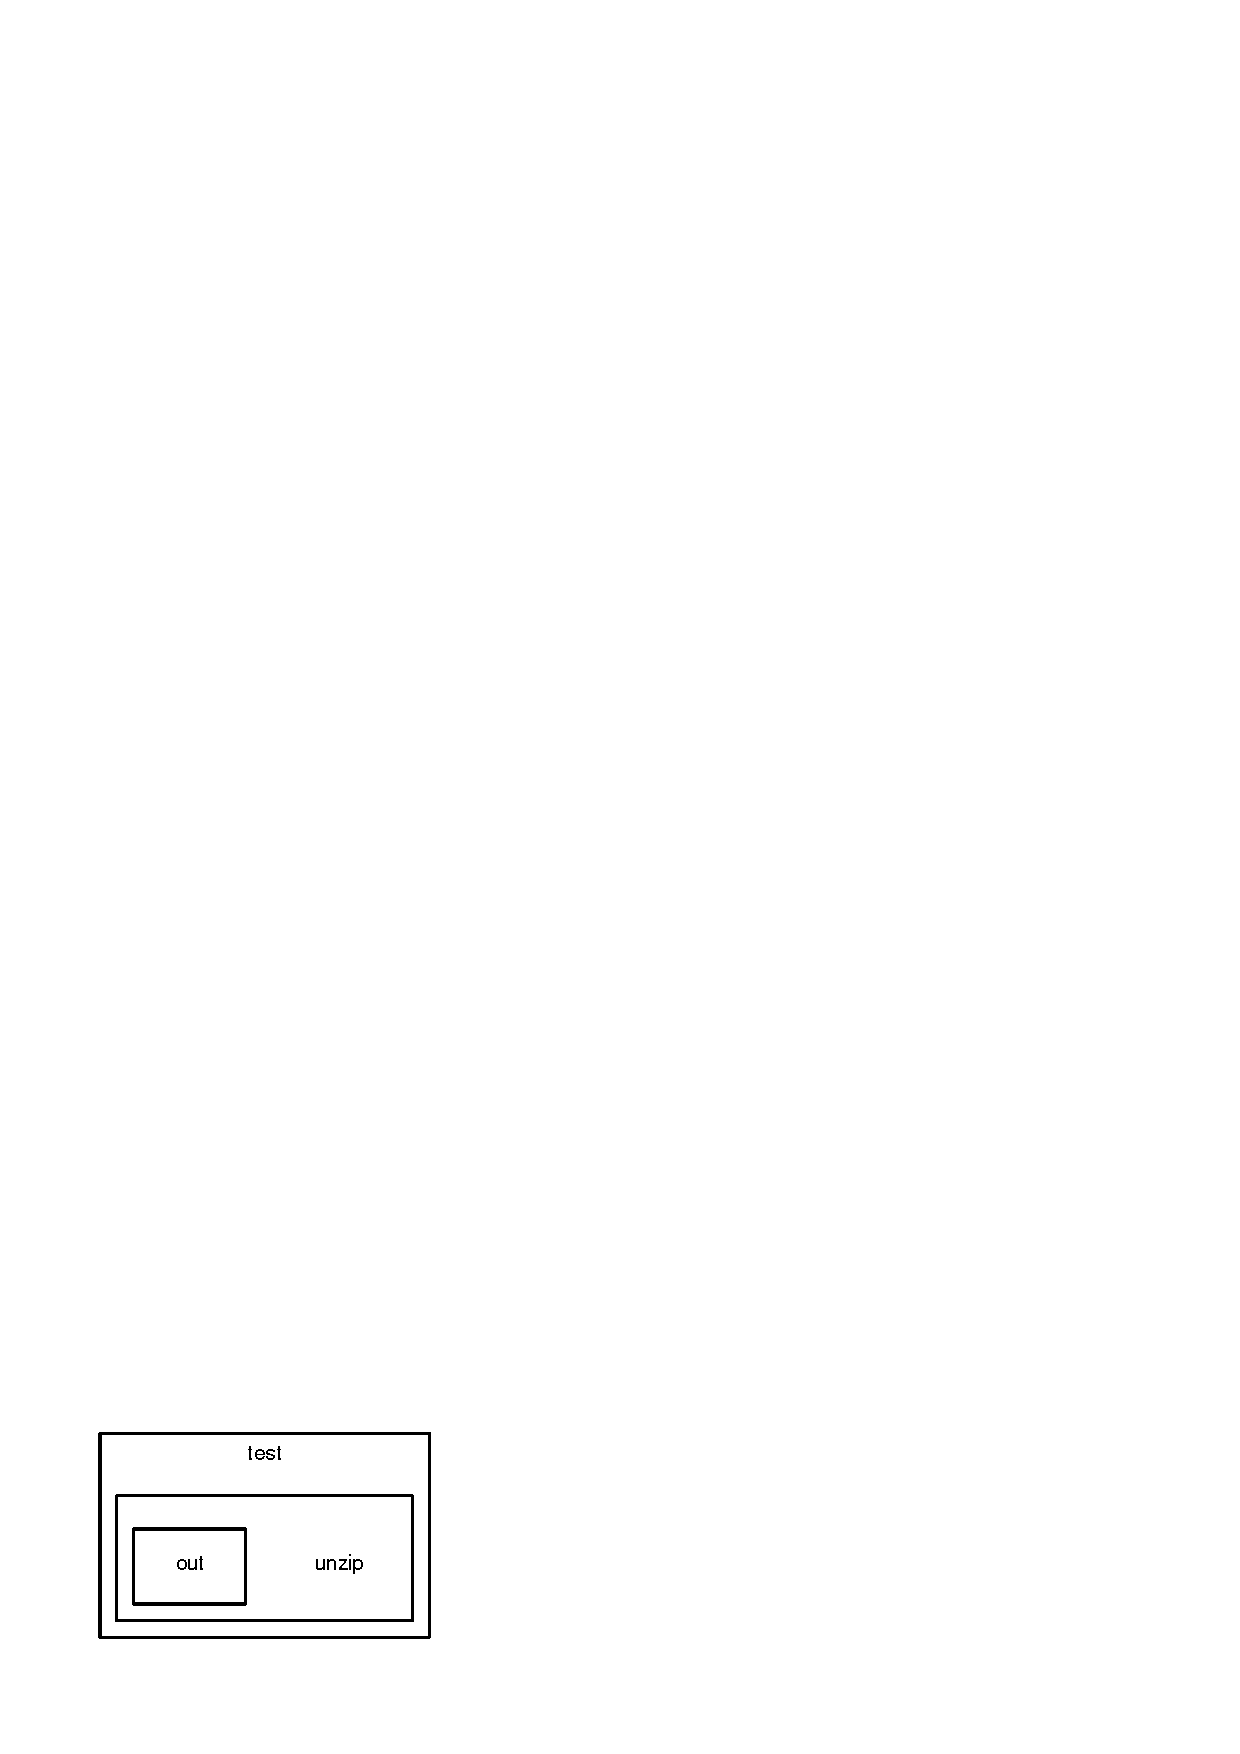
\includegraphics[width=109pt]{dir_0d290f915246044ba3a14f034cd1d91c_dep}
\end{center}
\end{figure}
\subsection*{Directories}
\begin{CompactItemize}
\item 
directory {\bf out}
\end{CompactItemize}
\subsection*{Files}
\begin{CompactItemize}
\item 
file \textbf{main.cpp}
\end{CompactItemize}

\section{test/zip/ Directory Reference}
\label{dir_ee4c44d0388c12031fb738965cf777e7}\index{test/zip/ Directory Reference@{test/zip/ Directory Reference}}


\nopagebreak
\begin{figure}[H]
\begin{center}
\leavevmode
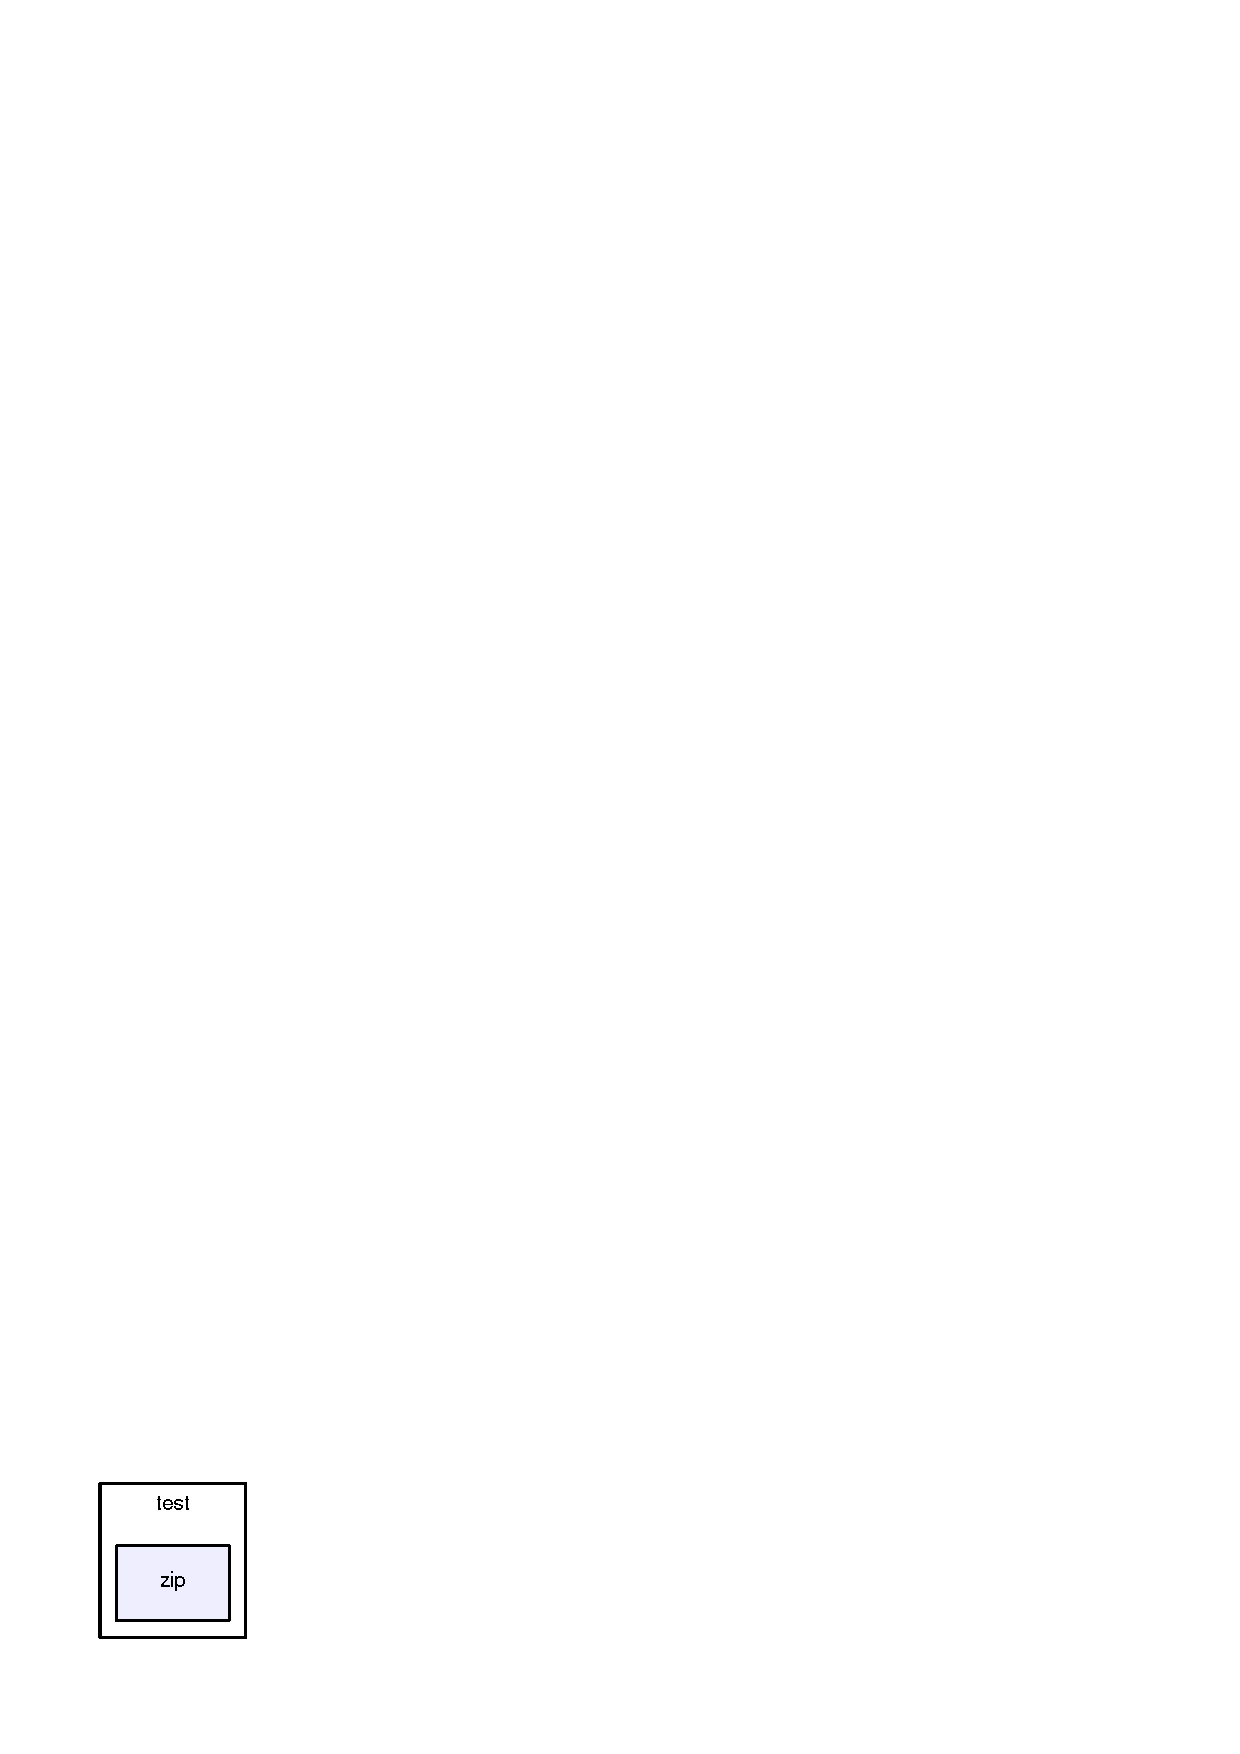
\includegraphics[width=65pt]{dir_ee4c44d0388c12031fb738965cf777e7_dep}
\end{center}
\end{figure}
\subsection*{Files}
\begin{CompactItemize}
\item 
file \textbf{main.cpp}
\end{CompactItemize}

\chapter{Class Documentation}
\section{QuaZip Class Reference}
\label{classQuaZip}\index{QuaZip@{QuaZip}}
ZIP archive.  


{\tt \#include $<$quazip/quazip.h$>$}

\subsection*{Public Types}
\begin{CompactItemize}
\item 
enum {\bf Constants} \{ {\bf MAX\_\-FILE\_\-NAME\_\-LENGTH} = 256
 \}
\begin{CompactList}\small\item\em Useful constants. \item\end{CompactList}\item 
enum {\bf Mode} \{ \par
{\bf mdNotOpen}, 
{\bf mdUnzip}, 
{\bf mdCreate}, 
{\bf mdAppend}, 
\par
{\bf mdAdd}
 \}
\begin{CompactList}\small\item\em Open mode of the ZIP file. \item\end{CompactList}\item 
enum {\bf CaseSensitivity} \{ {\bf csDefault} = 0, 
{\bf csSensitive} = 1, 
{\bf csInsensitive} = 2
 \}
\begin{CompactList}\small\item\em Case sensitivity for the file names. \item\end{CompactList}\end{CompactItemize}
\subsection*{Public Member Functions}
\begin{CompactItemize}
\item 
{\bf QuaZip} ()
\begin{CompactList}\small\item\em Constructs \doxyref{QuaZip}{p.}{classQuaZip} object. \item\end{CompactList}\item 
{\bf QuaZip} (const QString \&zipName)\label{classQuaZip_aea7294b02abd22379cc3a9fccb754b7}

\begin{CompactList}\small\item\em Constructs \doxyref{QuaZip}{p.}{classQuaZip} object associated with ZIP file {\em zipName\/}. \item\end{CompactList}\item 
{\bf $\sim$QuaZip} ()
\begin{CompactList}\small\item\em Destroys \doxyref{QuaZip}{p.}{classQuaZip} object. \item\end{CompactList}\item 
bool {\bf open} ({\bf Mode} mode, zlib\_\-filefunc\_\-def $\ast$ioApi=NULL)
\begin{CompactList}\small\item\em Opens ZIP file. \item\end{CompactList}\item 
void {\bf close} ()
\begin{CompactList}\small\item\em Closes ZIP file. \item\end{CompactList}\item 
void {\bf setFileNameCodec} (QTextCodec $\ast$fileNameCodec)
\begin{CompactList}\small\item\em Sets the codec used to encode/decode file names inside archive. \item\end{CompactList}\item 
void {\bf setFileNameCodec} (const char $\ast$fileNameCodecName)
\begin{CompactList}\small\item\em Sets the codec used to encode/decode file names inside archive. \item\end{CompactList}\item 
QTextCodec $\ast$ {\bf getFileNameCodec} () const \label{classQuaZip_c08a895376535a8860b9d5accd52e247}

\begin{CompactList}\small\item\em Returns the codec used to encode/decode comments inside archive. \item\end{CompactList}\item 
void {\bf setCommentCodec} (QTextCodec $\ast$commentCodec)
\begin{CompactList}\small\item\em Sets the codec used to encode/decode comments inside archive. \item\end{CompactList}\item 
void {\bf setCommentCodec} (const char $\ast$commentCodecName)
\begin{CompactList}\small\item\em Sets the codec used to encode/decode comments inside archive. \item\end{CompactList}\item 
QTextCodec $\ast$ {\bf getCommentCodec} () const \label{classQuaZip_25a8d6963e62eaff007569001e8715c4}

\begin{CompactList}\small\item\em Returns the codec used to encode/decode comments inside archive. \item\end{CompactList}\item 
QString {\bf getZipName} () const 
\begin{CompactList}\small\item\em Returns the name of the ZIP file. \item\end{CompactList}\item 
void {\bf setZipName} (const QString \&zipName)
\begin{CompactList}\small\item\em Sets the name of the ZIP file. \item\end{CompactList}\item 
{\bf Mode} {\bf getMode} () const \label{classQuaZip_5ad835fba0d8fb5a71f54c1ba7a4af4f}

\begin{CompactList}\small\item\em Returns the mode in which ZIP file was opened. \item\end{CompactList}\item 
bool {\bf isOpen} () const \label{classQuaZip_5b869a9c0d4f49955b759592fec08888}

\begin{CompactList}\small\item\em Returns {\tt true} if ZIP file is open, {\tt false} otherwise. \item\end{CompactList}\item 
int {\bf getZipError} () const 
\begin{CompactList}\small\item\em Returns the error code of the last operation. \item\end{CompactList}\item 
int {\bf getEntriesCount} () const 
\begin{CompactList}\small\item\em Returns number of the entries in the ZIP central directory. \item\end{CompactList}\item 
QString {\bf getComment} () const \label{classQuaZip_e55cfbf2296132df808c557b62433051}

\begin{CompactList}\small\item\em Returns global comment in the ZIP file. \item\end{CompactList}\item 
void {\bf setComment} (const QString \&comment)
\begin{CompactList}\small\item\em Sets global comment in the ZIP file. \item\end{CompactList}\item 
bool {\bf goToFirstFile} ()
\begin{CompactList}\small\item\em Sets the current file to the first file in the archive. \item\end{CompactList}\item 
bool {\bf goToNextFile} ()
\begin{CompactList}\small\item\em Sets the current file to the next file in the archive. \item\end{CompactList}\item 
bool {\bf setCurrentFile} (const QString \&fileName, {\bf CaseSensitivity} cs=csDefault)
\begin{CompactList}\small\item\em Sets current file by its name. \item\end{CompactList}\item 
bool {\bf hasCurrentFile} () const \label{classQuaZip_00b237d926648f45da86db25e7cfb697}

\begin{CompactList}\small\item\em Returns {\tt true} if the current file has been set. \item\end{CompactList}\item 
bool {\bf getCurrentFileInfo} ({\bf QuaZipFileInfo} $\ast$info) const 
\begin{CompactList}\small\item\em Retrieves information about the current file. \item\end{CompactList}\item 
QString {\bf getCurrentFileName} () const 
\begin{CompactList}\small\item\em Returns the current file name. \item\end{CompactList}\item 
unzFile {\bf getUnzFile} ()
\begin{CompactList}\small\item\em Returns {\tt unzFile} handle. \item\end{CompactList}\item 
zipFile {\bf getZipFile} ()
\begin{CompactList}\small\item\em Returns {\tt zipFile} handle. \item\end{CompactList}\end{CompactItemize}


\subsection{Detailed Description}
ZIP archive. 

This class implements basic interface to the ZIP archive. It can be used to read table contents of the ZIP archive and retreiving information about the files inside it.

You can also use this class to open files inside archive by passing pointer to the instance of this class to the constructor of the \doxyref{QuaZipFile}{p.}{classQuaZipFile} class. But see \doxyref{QuaZipFile::QuaZipFile(QuaZip$\ast$, QObject$\ast$)}{p.}{classQuaZipFile_54e944a6b3d27030f64c8f30d2cc33bb} for the possible pitfalls.

This class is indended to provide interface to the ZIP subpackage of the ZIP/UNZIP package as well as to the UNZIP subpackage. But currently it supports only UNZIP.

The use of this class is simple - just create instance using constructor, then set ZIP archive file name using setFile() function (if you did not passed the name to the constructor), then \doxyref{open()}{p.}{classQuaZip_bfa4e6018b2964a3d10a4c54e5ab3962} and then use different functions to work with it! Well, if you are paranoid, you may also wish to call close before destructing the instance, to check for errors on close.

You may also use \doxyref{getUnzFile()}{p.}{classQuaZip_3b78a652f296ff4a678a791e8294e642} and \doxyref{getZipFile()}{p.}{classQuaZip_425043a4d7cc31e2fe2bba73d954f15c} functions to get the ZIP archive handle and use it with ZIP/UNZIP package API directly.

This class supports localized file names inside ZIP archive, but you have to set up proper codec with setCodec() function. By default, locale codec will be used, which is probably ok for UNIX systems, but will almost certainly fail with ZIP archives created in Windows. This is because Windows ZIP programs have strange habit of using DOS encoding for file names in ZIP archives. For example, ZIP archive with cyrillic names created in Windows will have file names in {\tt IBM866} encoding instead of {\tt WINDOWS-1251}. I think that calling one function is not much trouble, but for true platform independency it would be nice to have some mechanism for file name encoding auto detection using locale information. Does anyone know a good way to do it? 

\subsection{Member Enumeration Documentation}
\index{QuaZip@{QuaZip}!Constants@{Constants}}
\index{Constants@{Constants}!QuaZip@{QuaZip}}
\subsubsection{\setlength{\rightskip}{0pt plus 5cm}enum {\bf QuaZip::Constants}}\label{classQuaZip_dce46b942c341dbb5c851eadead65459}


Useful constants. 

\begin{Desc}
\item[Enumerator: ]\par
\begin{description}
\index{MAX\_\-FILE\_\-NAME\_\-LENGTH@{MAX\_\-FILE\_\-NAME\_\-LENGTH}!QuaZip@{QuaZip}}\index{QuaZip@{QuaZip}!MAX\_\-FILE\_\-NAME\_\-LENGTH@{MAX\_\-FILE\_\-NAME\_\-LENGTH}}\item[{\em 
MAX\_\-FILE\_\-NAME\_\-LENGTH\label{classQuaZip_dce46b942c341dbb5c851eadead65459b26ce1a9c9e94f901dc2cf90fa5baa4b}
}]Maximum file name length. Taken from {\tt UNZ\_\-MAXFILENAMEINZIP} constant in unzip.c. \end{description}
\end{Desc}

\index{QuaZip@{QuaZip}!Mode@{Mode}}
\index{Mode@{Mode}!QuaZip@{QuaZip}}
\subsubsection{\setlength{\rightskip}{0pt plus 5cm}enum {\bf QuaZip::Mode}}\label{classQuaZip_47e28d4116ee716fdd6b431b821d0be4}


Open mode of the ZIP file. 

\begin{Desc}
\item[Enumerator: ]\par
\begin{description}
\index{mdNotOpen@{mdNotOpen}!QuaZip@{QuaZip}}\index{QuaZip@{QuaZip}!mdNotOpen@{mdNotOpen}}\item[{\em 
mdNotOpen\label{classQuaZip_47e28d4116ee716fdd6b431b821d0be4c87ddb1e901e1ec700c16ee0d4d398ce}
}]ZIP file is not open. This is the initial mode. \index{mdUnzip@{mdUnzip}!QuaZip@{QuaZip}}\index{QuaZip@{QuaZip}!mdUnzip@{mdUnzip}}\item[{\em 
mdUnzip\label{classQuaZip_47e28d4116ee716fdd6b431b821d0be4803a371910c2dc830d111e9ce5b58897}
}]ZIP file is open for reading files inside it. \index{mdCreate@{mdCreate}!QuaZip@{QuaZip}}\index{QuaZip@{QuaZip}!mdCreate@{mdCreate}}\item[{\em 
mdCreate\label{classQuaZip_47e28d4116ee716fdd6b431b821d0be425ae05b12590540af8c66ae8298b928e}
}]ZIP file was created with \doxyref{open()}{p.}{classQuaZip_bfa4e6018b2964a3d10a4c54e5ab3962} call. \index{mdAppend@{mdAppend}!QuaZip@{QuaZip}}\index{QuaZip@{QuaZip}!mdAppend@{mdAppend}}\item[{\em 
mdAppend\label{classQuaZip_47e28d4116ee716fdd6b431b821d0be4b807f0c65653a16d77b365801fd25582}
}]ZIP file was opened in append mode. This refers to {\tt APPEND\_\-STATUS\_\-CREATEAFTER} mode in ZIP/UNZIP package and means that zip is appended to some existing file what is useful when that file contains self-extractor code. This is obviously {\em not\/} what you whant to use to add files to the existing ZIP archive. \index{mdAdd@{mdAdd}!QuaZip@{QuaZip}}\index{QuaZip@{QuaZip}!mdAdd@{mdAdd}}\item[{\em 
mdAdd\label{classQuaZip_47e28d4116ee716fdd6b431b821d0be422c745f349f06add449af523254fdaec}
}]ZIP file was opened for adding files in the archive. \end{description}
\end{Desc}

\index{QuaZip@{QuaZip}!CaseSensitivity@{CaseSensitivity}}
\index{CaseSensitivity@{CaseSensitivity}!QuaZip@{QuaZip}}
\subsubsection{\setlength{\rightskip}{0pt plus 5cm}enum {\bf QuaZip::CaseSensitivity}}\label{classQuaZip_6053a1d249ed210a85c9d5eb7cf9cdbe}


Case sensitivity for the file names. 

This is what you specify when accessing files in the archive. Works perfectly fine with any characters thanks to Qt's great unicode support. This is different from ZIP/UNZIP API, where only US-ASCII characters was supported. \begin{Desc}
\item[Enumerator: ]\par
\begin{description}
\index{csDefault@{csDefault}!QuaZip@{QuaZip}}\index{QuaZip@{QuaZip}!csDefault@{csDefault}}\item[{\em 
csDefault\label{classQuaZip_6053a1d249ed210a85c9d5eb7cf9cdbec3cca8c0b976cf6397a28a5c84e75253}
}]Default for platform. Case sensitive for UNIX, not for Windows. \index{csSensitive@{csSensitive}!QuaZip@{QuaZip}}\index{QuaZip@{QuaZip}!csSensitive@{csSensitive}}\item[{\em 
csSensitive\label{classQuaZip_6053a1d249ed210a85c9d5eb7cf9cdbed8d86b0c34203336cad09348cfa5356e}
}]Case sensitive. \index{csInsensitive@{csInsensitive}!QuaZip@{QuaZip}}\index{QuaZip@{QuaZip}!csInsensitive@{csInsensitive}}\item[{\em 
csInsensitive\label{classQuaZip_6053a1d249ed210a85c9d5eb7cf9cdbe3e492bcc3f64f41a74906cecc45fb366}
}]Case insensitive. \end{description}
\end{Desc}



\subsection{Constructor \& Destructor Documentation}
\index{QuaZip@{QuaZip}!QuaZip@{QuaZip}}
\index{QuaZip@{QuaZip}!QuaZip@{QuaZip}}
\subsubsection{\setlength{\rightskip}{0pt plus 5cm}QuaZip::QuaZip ()}\label{classQuaZip_970e0f401c7cfd7a78e78572f758eec4}


Constructs \doxyref{QuaZip}{p.}{classQuaZip} object. 

Call setName() before opening constructed object. \index{QuaZip@{QuaZip}!$\sim$QuaZip@{$\sim$QuaZip}}
\index{$\sim$QuaZip@{$\sim$QuaZip}!QuaZip@{QuaZip}}
\subsubsection{\setlength{\rightskip}{0pt plus 5cm}QuaZip::$\sim$QuaZip ()}\label{classQuaZip_f60a2d3930b90f3b25a3148baecad81e}


Destroys \doxyref{QuaZip}{p.}{classQuaZip} object. 

Calls \doxyref{close()}{p.}{classQuaZip_7a4323b73e12f3b4470109f200728f9f} if necessary. 

References close(), and isOpen().

\subsection{Member Function Documentation}
\index{QuaZip@{QuaZip}!open@{open}}
\index{open@{open}!QuaZip@{QuaZip}}
\subsubsection{\setlength{\rightskip}{0pt plus 5cm}bool QuaZip::open ({\bf Mode} {\em mode}, \/  zlib\_\-filefunc\_\-def $\ast$ {\em ioApi} = {\tt NULL})}\label{classQuaZip_bfa4e6018b2964a3d10a4c54e5ab3962}


Opens ZIP file. 

Argument {\em ioApi\/} specifies IO function set for ZIP/UNZIP package to use. See unzip.h, zip.h and ioapi.h for details. By passing NULL (the default) you just tell package to use the default API which works just fine on UNIX platforms. I have tried it on win32-g++ platform too and it seems it works fine there too, so I see no reason to use win32 IO API included in original ZIP/UNZIP package.

ZIP archive file name will be converted to 8-bit encoding using Qt's QFile::encodeName() function before passing it to the ZIP/UNZIP package API.

Returns {\tt true} if successful, {\tt false} otherwise.

Argument {\em mode\/} specifies open mode of the ZIP archive. See Mode for details. Note that there is zipOpen2() function in the ZIP/UNZIP API which accepts {\em globalcomment\/} argument, but it does not use it anywhere, so this \doxyref{open()}{p.}{classQuaZip_bfa4e6018b2964a3d10a4c54e5ab3962} function does not have this argument. See \doxyref{setComment()}{p.}{classQuaZip_1b5d936a203859340574d5908ffa2222} if you need to set global comment.

\begin{Desc}
\item[Note:]ZIP/UNZIP API open calls do not return error code - they just return {\tt NULL} indicating an error. But to make things easier, \doxyref{quazip.h}{p.}{quazip_8h-source} header defines additional error code {\tt UNZ\_\-ERROROPEN} and \doxyref{getZipError()}{p.}{classQuaZip_28b91a6282ddd9382c96a069572c6fb4} will return it if the open call of the ZIP/UNZIP API returns {\tt NULL}. \end{Desc}


References isOpen(), mdAdd, mdAppend, mdCreate, and mdUnzip.

Referenced by QuaZipFile::open().\index{QuaZip@{QuaZip}!close@{close}}
\index{close@{close}!QuaZip@{QuaZip}}
\subsubsection{\setlength{\rightskip}{0pt plus 5cm}void QuaZip::close ()}\label{classQuaZip_7a4323b73e12f3b4470109f200728f9f}


Closes ZIP file. 

Call \doxyref{getZipError()}{p.}{classQuaZip_28b91a6282ddd9382c96a069572c6fb4} to determine if the close was successful. 

References mdAdd, mdAppend, mdCreate, mdNotOpen, and mdUnzip.

Referenced by QuaZipFile::close(), QuaZipFile::open(), and $\sim$QuaZip().\index{QuaZip@{QuaZip}!setFileNameCodec@{setFileNameCodec}}
\index{setFileNameCodec@{setFileNameCodec}!QuaZip@{QuaZip}}
\subsubsection{\setlength{\rightskip}{0pt plus 5cm}void QuaZip::setFileNameCodec (QTextCodec $\ast$ {\em fileNameCodec})\hspace{0.3cm}{\tt  [inline]}}\label{classQuaZip_339010b5566704ba3c9cafbfe848d8fb}


Sets the codec used to encode/decode file names inside archive. 

This is necessary to access files in the ZIP archive created under Windows with non-latin characters in file names. For example, file names with cyrillic letters will be in {\tt IBM866} encoding. \index{QuaZip@{QuaZip}!setFileNameCodec@{setFileNameCodec}}
\index{setFileNameCodec@{setFileNameCodec}!QuaZip@{QuaZip}}
\subsubsection{\setlength{\rightskip}{0pt plus 5cm}void QuaZip::setFileNameCodec (const char $\ast$ {\em fileNameCodecName})\hspace{0.3cm}{\tt  [inline]}}\label{classQuaZip_8f283519a195aa1d9076bbbb01ea0497}


Sets the codec used to encode/decode file names inside archive. 

This is an overloaded member function, provided for convenience. It differs from the above function only in what argument(s) it accepts. Equivalent to calling setFileNameCodec(QTextCodec::codecForName(codecName)); \index{QuaZip@{QuaZip}!setCommentCodec@{setCommentCodec}}
\index{setCommentCodec@{setCommentCodec}!QuaZip@{QuaZip}}
\subsubsection{\setlength{\rightskip}{0pt plus 5cm}void QuaZip::setCommentCodec (QTextCodec $\ast$ {\em commentCodec})\hspace{0.3cm}{\tt  [inline]}}\label{classQuaZip_1c81fca7215a4374f6f03872ade4885b}


Sets the codec used to encode/decode comments inside archive. 

This codec defaults to locale codec, which is probably ok. \index{QuaZip@{QuaZip}!setCommentCodec@{setCommentCodec}}
\index{setCommentCodec@{setCommentCodec}!QuaZip@{QuaZip}}
\subsubsection{\setlength{\rightskip}{0pt plus 5cm}void QuaZip::setCommentCodec (const char $\ast$ {\em commentCodecName})\hspace{0.3cm}{\tt  [inline]}}\label{classQuaZip_413f3c56b54a9a47258d53802cb606e7}


Sets the codec used to encode/decode comments inside archive. 

This is an overloaded member function, provided for convenience. It differs from the above function only in what argument(s) it accepts. Equivalent to calling setCommentCodec(QTextCodec::codecForName(codecName)); \index{QuaZip@{QuaZip}!getZipName@{getZipName}}
\index{getZipName@{getZipName}!QuaZip@{QuaZip}}
\subsubsection{\setlength{\rightskip}{0pt plus 5cm}QString QuaZip::getZipName () const\hspace{0.3cm}{\tt  [inline]}}\label{classQuaZip_4f7deef08ff40aeb1a7a04bcd7f228c2}


Returns the name of the ZIP file. 

Returns null string if no ZIP file name has been set. \begin{Desc}
\item[See also:]\doxyref{setZipName()}{p.}{classQuaZip_a80b661de1262af905d1677dbcb008cc} \end{Desc}


Referenced by QuaZipFile::getZipName().\index{QuaZip@{QuaZip}!setZipName@{setZipName}}
\index{setZipName@{setZipName}!QuaZip@{QuaZip}}
\subsubsection{\setlength{\rightskip}{0pt plus 5cm}void QuaZip::setZipName (const QString \& {\em zipName})}\label{classQuaZip_a80b661de1262af905d1677dbcb008cc}


Sets the name of the ZIP file. 

Does nothing if the ZIP file is open.

Does not reset error code returned by \doxyref{getZipError()}{p.}{classQuaZip_28b91a6282ddd9382c96a069572c6fb4}. 

References isOpen().\index{QuaZip@{QuaZip}!getZipError@{getZipError}}
\index{getZipError@{getZipError}!QuaZip@{QuaZip}}
\subsubsection{\setlength{\rightskip}{0pt plus 5cm}int QuaZip::getZipError () const\hspace{0.3cm}{\tt  [inline]}}\label{classQuaZip_28b91a6282ddd9382c96a069572c6fb4}


Returns the error code of the last operation. 

Returns {\tt UNZ\_\-OK} if the last operation was successful.

Error code resets to {\tt UNZ\_\-OK} every time you call any function that accesses something inside ZIP archive, even if it is {\tt const} (like \doxyref{getEntriesCount()}{p.}{classQuaZip_2ea4bd1fca948637c35c2d2752bb5a80}). \doxyref{open()}{p.}{classQuaZip_bfa4e6018b2964a3d10a4c54e5ab3962} and \doxyref{close()}{p.}{classQuaZip_7a4323b73e12f3b4470109f200728f9f} calls reset error code too. See documentation for the specific functions for details on error detection. 

Referenced by QuaZipFile::close(), QuaZipFile::getActualFileName(), QuaZipFile::getFileInfo(), and QuaZipFile::open().\index{QuaZip@{QuaZip}!getEntriesCount@{getEntriesCount}}
\index{getEntriesCount@{getEntriesCount}!QuaZip@{QuaZip}}
\subsubsection{\setlength{\rightskip}{0pt plus 5cm}int QuaZip::getEntriesCount () const}\label{classQuaZip_2ea4bd1fca948637c35c2d2752bb5a80}


Returns number of the entries in the ZIP central directory. 

Returns negative error code in the case of error. The same error code will be returned by subsequent \doxyref{getZipError()}{p.}{classQuaZip_28b91a6282ddd9382c96a069572c6fb4} call. 

References mdUnzip, and zipError.\index{QuaZip@{QuaZip}!setComment@{setComment}}
\index{setComment@{setComment}!QuaZip@{QuaZip}}
\subsubsection{\setlength{\rightskip}{0pt plus 5cm}void QuaZip::setComment (const QString \& {\em comment})\hspace{0.3cm}{\tt  [inline]}}\label{classQuaZip_1b5d936a203859340574d5908ffa2222}


Sets global comment in the ZIP file. 

Comment will be written to the archive on close operation.

\begin{Desc}
\item[See also:]\doxyref{open()}{p.}{classQuaZip_bfa4e6018b2964a3d10a4c54e5ab3962} \end{Desc}
\index{QuaZip@{QuaZip}!goToFirstFile@{goToFirstFile}}
\index{goToFirstFile@{goToFirstFile}!QuaZip@{QuaZip}}
\subsubsection{\setlength{\rightskip}{0pt plus 5cm}bool QuaZip::goToFirstFile ()}\label{classQuaZip_745488f9177bcec3cdb858587584e033}


Sets the current file to the first file in the archive. 

Returns {\tt true} on success, {\tt false} otherwise. Call \doxyref{getZipError()}{p.}{classQuaZip_28b91a6282ddd9382c96a069572c6fb4} to get the error code. 

References mdUnzip.

Referenced by setCurrentFile().\index{QuaZip@{QuaZip}!goToNextFile@{goToNextFile}}
\index{goToNextFile@{goToNextFile}!QuaZip@{QuaZip}}
\subsubsection{\setlength{\rightskip}{0pt plus 5cm}bool QuaZip::goToNextFile ()}\label{classQuaZip_ee6779b6cd338420c2e8c5655fa8ba97}


Sets the current file to the next file in the archive. 

Returns {\tt true} on success, {\tt false} otherwise. Call \doxyref{getZipError()}{p.}{classQuaZip_28b91a6282ddd9382c96a069572c6fb4} to determine if there was an error.

Should be used only in \doxyref{QuaZip::mdUnzip}{p.}{classQuaZip_47e28d4116ee716fdd6b431b821d0be4803a371910c2dc830d111e9ce5b58897} mode.

\begin{Desc}
\item[Note:]If the end of file was reached, \doxyref{getZipError()}{p.}{classQuaZip_28b91a6282ddd9382c96a069572c6fb4} will return {\tt UNZ\_\-OK} instead of {\tt UNZ\_\-END\_\-OF\_\-LIST\_\-OF\_\-FILE}. This is to make things like this easier: 

\begin{Code}\begin{verbatim} for(bool more=zip.goToFirstFile(); more; more=zip.goToNextFile()) {
   // do something
 }
 if(zip.getZipError()==UNZ_OK) {
   // ok, there was no error
 }
\end{verbatim}
\end{Code}

 \end{Desc}


References mdUnzip.

Referenced by setCurrentFile().\index{QuaZip@{QuaZip}!setCurrentFile@{setCurrentFile}}
\index{setCurrentFile@{setCurrentFile}!QuaZip@{QuaZip}}
\subsubsection{\setlength{\rightskip}{0pt plus 5cm}bool QuaZip::setCurrentFile (const QString \& {\em fileName}, \/  {\bf CaseSensitivity} {\em cs} = {\tt csDefault})}\label{classQuaZip_6c657bfcfccb59d728e0da24c677d899}


Sets current file by its name. 

Returns {\tt true} if successful, {\tt false} otherwise. Argument {\em cs\/} specifies case sensitivity of the file name. Call \doxyref{getZipError()}{p.}{classQuaZip_28b91a6282ddd9382c96a069572c6fb4} in the case of a failure to get error code.

This is not a wrapper to unzLocateFile() function. That is because I had to implement locale-specific case-insensitive comparison.

Here are the differences from the original implementation:

\begin{itemize}
\item If the file was not found, error code is {\tt UNZ\_\-OK}, not {\tt UNZ\_\-END\_\-OF\_\-LIST\_\-OF\_\-FILE} (see also \doxyref{goToNextFile()}{p.}{classQuaZip_ee6779b6cd338420c2e8c5655fa8ba97}).\item If this function fails, it unsets the current file rather than resetting it back to what it was before the call.\end{itemize}


If {\em fileName\/} is null string then this function unsets the current file and return {\tt true}. Note that you should close the file first if it is open! See \doxyref{QuaZipFile::QuaZipFile(QuaZip$\ast$,QObject$\ast$)}{p.}{classQuaZipFile_54e944a6b3d27030f64c8f30d2cc33bb} for the details.

Should be used only in \doxyref{QuaZip::mdUnzip}{p.}{classQuaZip_47e28d4116ee716fdd6b431b821d0be4803a371910c2dc830d111e9ce5b58897} mode.

\begin{Desc}
\item[See also:]\doxyref{setFileNameCodec()}{p.}{classQuaZip_339010b5566704ba3c9cafbfe848d8fb}, \doxyref{CaseSensitivity}{p.}{classQuaZip_6053a1d249ed210a85c9d5eb7cf9cdbe} \end{Desc}


References csDefault, csSensitive, getCurrentFileName(), goToFirstFile(), goToNextFile(), MAX\_\-FILE\_\-NAME\_\-LENGTH, and mdUnzip.

Referenced by QuaZipFile::open().\index{QuaZip@{QuaZip}!getCurrentFileInfo@{getCurrentFileInfo}}
\index{getCurrentFileInfo@{getCurrentFileInfo}!QuaZip@{QuaZip}}
\subsubsection{\setlength{\rightskip}{0pt plus 5cm}bool QuaZip::getCurrentFileInfo ({\bf QuaZipFileInfo} $\ast$ {\em info}) const}\label{classQuaZip_9c91a53ed4c2038e153c64bdc097ebe8}


Retrieves information about the current file. 

Fills the structure pointed by {\em info\/}. Returns {\tt true} on success, {\tt false} otherwise. In the latter case structure pointed by {\em info\/} remains untouched. If there was an error, \doxyref{getZipError()}{p.}{classQuaZip_28b91a6282ddd9382c96a069572c6fb4} returns error code.

Should be used only in \doxyref{QuaZip::mdUnzip}{p.}{classQuaZip_47e28d4116ee716fdd6b431b821d0be4803a371910c2dc830d111e9ce5b58897} mode.

Does nothing and returns {\tt false} in any of the following cases.\begin{itemize}
\item ZIP is not open;\item ZIP does not have current file;\item {\em info\/} is {\tt NULL};\end{itemize}


In all these cases \doxyref{getZipError()}{p.}{classQuaZip_28b91a6282ddd9382c96a069572c6fb4} returns {\tt UNZ\_\-OK} since there is no ZIP/UNZIP API call. 

References QuaZipFileInfo::comment, QuaZipFileInfo::compressedSize, QuaZipFileInfo::crc, QuaZipFileInfo::dateTime, QuaZipFileInfo::diskNumberStart, QuaZipFileInfo::externalAttr, QuaZipFileInfo::extra, QuaZipFileInfo::flags, hasCurrentFile(), QuaZipFileInfo::internalAttr, isOpen(), mdUnzip, QuaZipFileInfo::method, QuaZipFileInfo::name, QuaZipFileInfo::uncompressedSize, QuaZipFileInfo::versionCreated, QuaZipFileInfo::versionNeeded, and zipError.

Referenced by QuaZipFile::getFileInfo().\index{QuaZip@{QuaZip}!getCurrentFileName@{getCurrentFileName}}
\index{getCurrentFileName@{getCurrentFileName}!QuaZip@{QuaZip}}
\subsubsection{\setlength{\rightskip}{0pt plus 5cm}QString QuaZip::getCurrentFileName () const}\label{classQuaZip_9783f8b4f39cd55e71e975aea78fd54a}


Returns the current file name. 

Equivalent to calling \doxyref{getCurrentFileInfo()}{p.}{classQuaZip_9c91a53ed4c2038e153c64bdc097ebe8} and then getting {\tt name} field of the \doxyref{QuaZipFileInfo}{p.}{structQuaZipFileInfo} structure, but faster and more convenient.

Should be used only in \doxyref{QuaZip::mdUnzip}{p.}{classQuaZip_47e28d4116ee716fdd6b431b821d0be4803a371910c2dc830d111e9ce5b58897} mode. 

References hasCurrentFile(), isOpen(), MAX\_\-FILE\_\-NAME\_\-LENGTH, mdUnzip, and zipError.

Referenced by QuaZipFile::getActualFileName(), and setCurrentFile().\index{QuaZip@{QuaZip}!getUnzFile@{getUnzFile}}
\index{getUnzFile@{getUnzFile}!QuaZip@{QuaZip}}
\subsubsection{\setlength{\rightskip}{0pt plus 5cm}unzFile QuaZip::getUnzFile ()\hspace{0.3cm}{\tt  [inline]}}\label{classQuaZip_3b78a652f296ff4a678a791e8294e642}


Returns {\tt unzFile} handle. 

You can use this handle to directly call UNZIP part of the ZIP/UNZIP package functions (see unzip.h).

\begin{Desc}
\item[Warning:]When using the handle returned by this function, please keep in mind that \doxyref{QuaZip}{p.}{classQuaZip} class is unable to detect any changes you make in the ZIP file state (e. g. changing current file, or closing the handle). So please do not do anything with this handle that is possible to do with the functions of this class. Or at least return the handle in the original state before calling some another function of this class (including implicit destructor calls and calls from the \doxyref{QuaZipFile}{p.}{classQuaZipFile} objects that refer to this \doxyref{QuaZip}{p.}{classQuaZip} instance!). So if you have changed the current file in the ZIP archive - then change it back or you may experience some strange behavior or even crashes. \end{Desc}


Referenced by QuaZipFile::atEnd(), QuaZipFile::close(), QuaZipFile::csize(), QuaZipFile::open(), QuaZipFile::pos(), QuaZipFile::readData(), and QuaZipFile::usize().\index{QuaZip@{QuaZip}!getZipFile@{getZipFile}}
\index{getZipFile@{getZipFile}!QuaZip@{QuaZip}}
\subsubsection{\setlength{\rightskip}{0pt plus 5cm}zipFile QuaZip::getZipFile ()\hspace{0.3cm}{\tt  [inline]}}\label{classQuaZip_425043a4d7cc31e2fe2bba73d954f15c}


Returns {\tt zipFile} handle. 

You can use this handle to directly call ZIP part of the ZIP/UNZIP package functions (see zip.h). Warnings about the \doxyref{getUnzFile()}{p.}{classQuaZip_3b78a652f296ff4a678a791e8294e642} function also apply to this function. 

Referenced by QuaZipFile::close(), QuaZipFile::open(), and QuaZipFile::writeData().

The documentation for this class was generated from the following files:\begin{CompactItemize}
\item 
quazip/quazip.h\item 
quazip/quazip.cpp\end{CompactItemize}

\section{QuaZipFile Class Reference}
\label{classQuaZipFile}\index{QuaZipFile@{QuaZipFile}}
A file inside ZIP archive.  


{\tt \#include $<$quazip/quazipfile.h$>$}

Collaboration diagram for QuaZipFile:\nopagebreak
\begin{figure}[H]
\begin{center}
\leavevmode
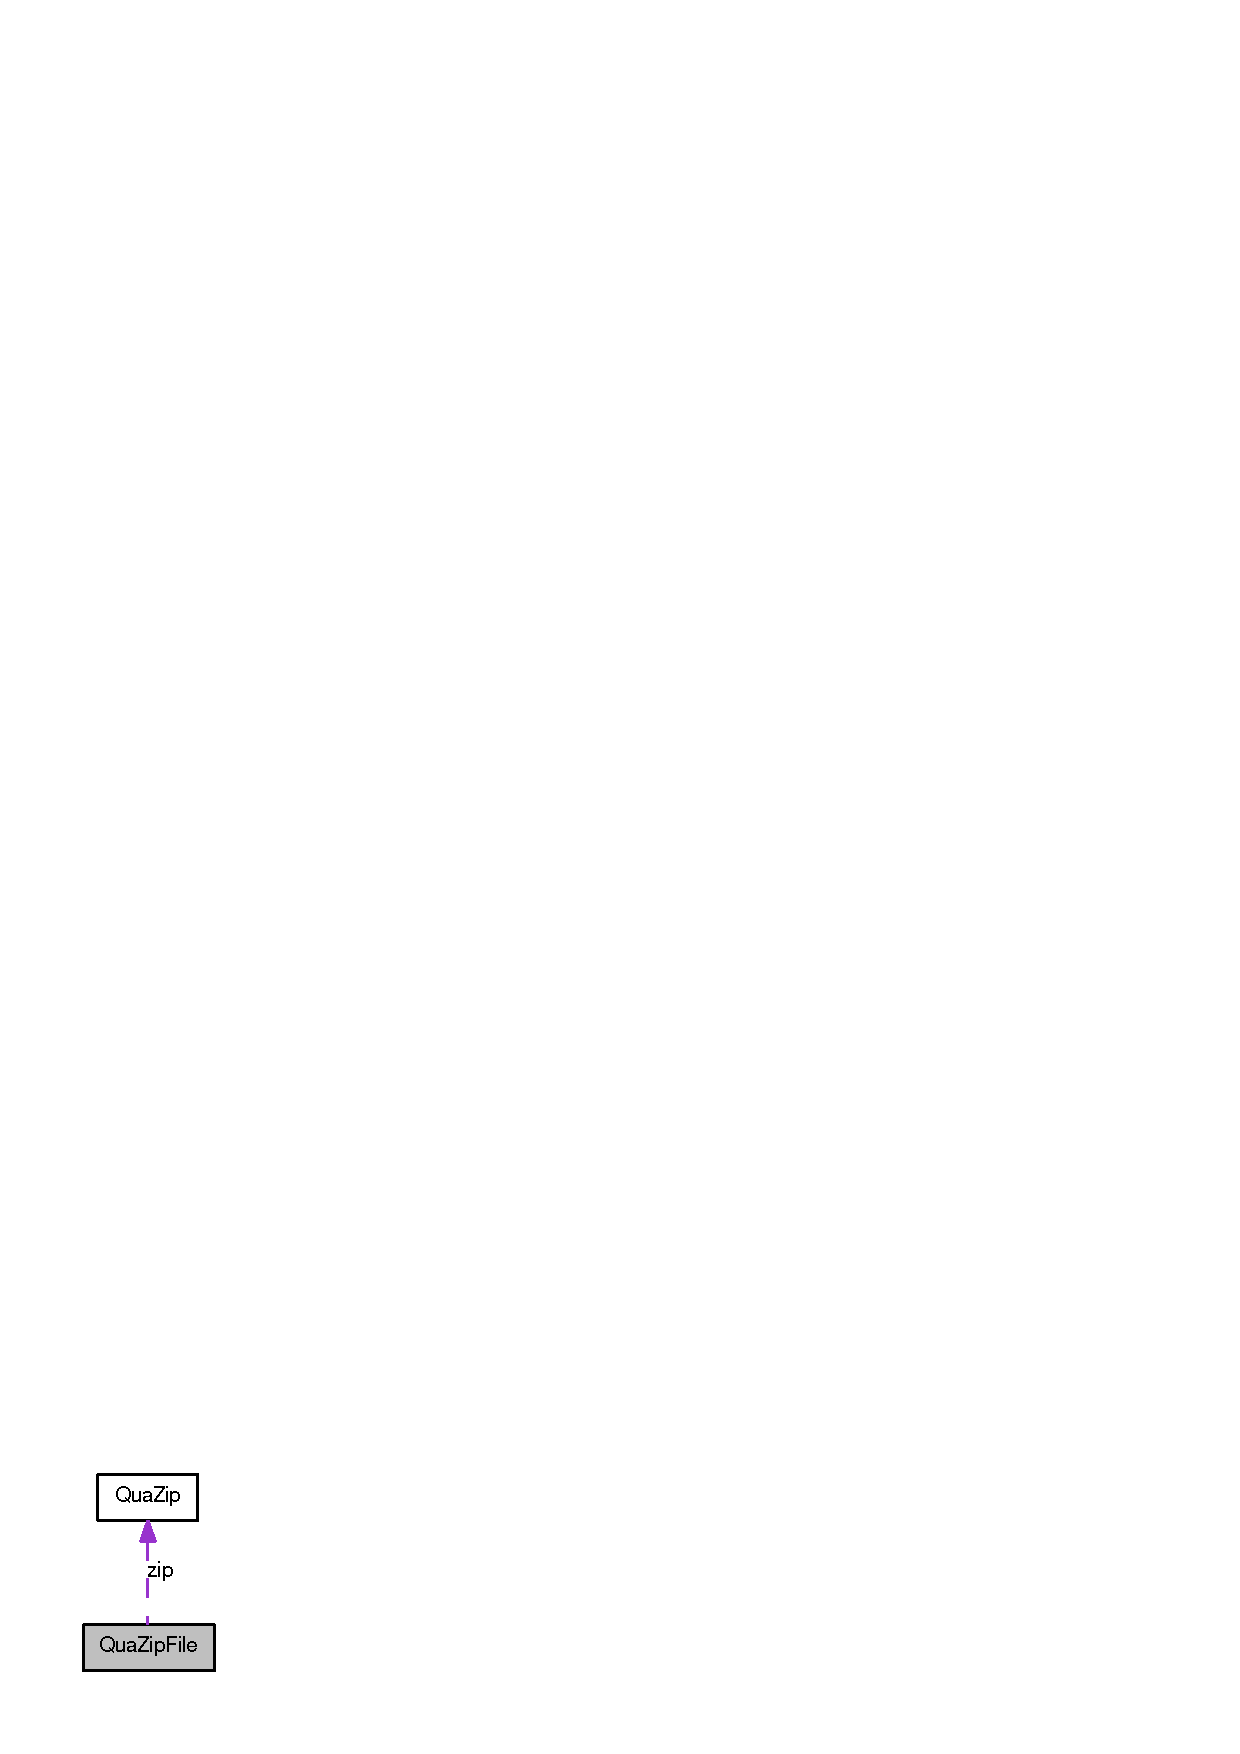
\includegraphics[width=53pt]{classQuaZipFile__coll__graph}
\end{center}
\end{figure}
\subsection*{Public Member Functions}
\begin{CompactItemize}
\item 
{\bf QuaZipFile} ()
\begin{CompactList}\small\item\em Constructs a \doxyref{QuaZipFile}{p.}{classQuaZipFile} instance. \item\end{CompactList}\item 
{\bf QuaZipFile} (QObject $\ast$parent)
\begin{CompactList}\small\item\em Constructs a \doxyref{QuaZipFile}{p.}{classQuaZipFile} instance. \item\end{CompactList}\item 
{\bf QuaZipFile} (const QString \&zipName, QObject $\ast$parent=NULL)
\begin{CompactList}\small\item\em Constructs a \doxyref{QuaZipFile}{p.}{classQuaZipFile} instance. \item\end{CompactList}\item 
{\bf QuaZipFile} (const QString \&zipName, const QString \&fileName, {\bf QuaZip::CaseSensitivity} cs=QuaZip::csDefault, QObject $\ast$parent=NULL)
\begin{CompactList}\small\item\em Constructs a \doxyref{QuaZipFile}{p.}{classQuaZipFile} instance. \item\end{CompactList}\item 
{\bf QuaZipFile} ({\bf QuaZip} $\ast$zip, QObject $\ast$parent=NULL)
\begin{CompactList}\small\item\em Constructs a \doxyref{QuaZipFile}{p.}{classQuaZipFile} instance. \item\end{CompactList}\item 
virtual {\bf $\sim$QuaZipFile} ()
\begin{CompactList}\small\item\em Destroys a \doxyref{QuaZipFile}{p.}{classQuaZipFile} instance. \item\end{CompactList}\item 
QString {\bf getZipName} () const 
\begin{CompactList}\small\item\em Returns the ZIP archive file name. \item\end{CompactList}\item 
{\bf QuaZip} $\ast$ {\bf getZip} () const 
\begin{CompactList}\small\item\em Returns a pointer to the associated \doxyref{QuaZip}{p.}{classQuaZip} object. \item\end{CompactList}\item 
QString {\bf getFileName} () const 
\begin{CompactList}\small\item\em Returns file name. \item\end{CompactList}\item 
{\bf QuaZip::CaseSensitivity} {\bf getCaseSensitivity} () const 
\begin{CompactList}\small\item\em Returns case sensitivity of the file name. \item\end{CompactList}\item 
QString {\bf getActualFileName} () const 
\begin{CompactList}\small\item\em Returns the actual file name in the archive. \item\end{CompactList}\item 
void {\bf setZipName} (const QString \&zipName)
\begin{CompactList}\small\item\em Sets the ZIP archive file name. \item\end{CompactList}\item 
bool {\bf isRaw} () const 
\begin{CompactList}\small\item\em Returns {\tt true} if the file was opened in raw mode. \item\end{CompactList}\item 
void {\bf setZip} ({\bf QuaZip} $\ast$zip)
\begin{CompactList}\small\item\em Binds to the existing \doxyref{QuaZip}{p.}{classQuaZip} instance. \item\end{CompactList}\item 
void {\bf setFileName} (const QString \&fileName, {\bf QuaZip::CaseSensitivity} cs=QuaZip::csDefault)
\begin{CompactList}\small\item\em Sets the file name. \item\end{CompactList}\item 
virtual bool {\bf open} (OpenMode mode)
\begin{CompactList}\small\item\em Opens a file for reading. \item\end{CompactList}\item 
bool {\bf open} (OpenMode mode, const char $\ast$password)
\begin{CompactList}\small\item\em Opens a file for reading. \item\end{CompactList}\item 
bool {\bf open} (OpenMode mode, int $\ast$method, int $\ast$level, bool raw, const char $\ast$password=NULL)
\begin{CompactList}\small\item\em Opens a file for reading. \item\end{CompactList}\item 
bool {\bf open} (OpenMode mode, const {\bf QuaZipNewInfo} \&info, const char $\ast$password=NULL, quint32 crc=0, int method=Z\_\-DEFLATED, int level=Z\_\-DEFAULT\_\-COMPRESSION, bool raw=false, int windowBits=-MAX\_\-WBITS, int memLevel=DEF\_\-MEM\_\-LEVEL, int strategy=Z\_\-DEFAULT\_\-STRATEGY)
\begin{CompactList}\small\item\em Opens a file for writing. \item\end{CompactList}\item 
virtual bool {\bf isSequential} () const \label{classQuaZipFile_64430ec50820c8096f963a7e5f53001f}

\begin{CompactList}\small\item\em Returns {\tt true}, but \doxyref{beware}{p.}{classQuaZipFile_quazipfile-sequential}! \item\end{CompactList}\item 
virtual qint64 {\bf pos} () const 
\begin{CompactList}\small\item\em Returns current position in the file. \item\end{CompactList}\item 
virtual bool {\bf atEnd} () const 
\begin{CompactList}\small\item\em Returns {\tt true} if the end of file was reached. \item\end{CompactList}\item 
virtual qint64 {\bf size} () const 
\begin{CompactList}\small\item\em Returns file size. \item\end{CompactList}\item 
qint64 {\bf csize} () const 
\begin{CompactList}\small\item\em Returns compressed file size. \item\end{CompactList}\item 
qint64 {\bf usize} () const 
\begin{CompactList}\small\item\em Returns uncompressed file size. \item\end{CompactList}\item 
bool {\bf getFileInfo} ({\bf QuaZipFileInfo} $\ast$info)
\begin{CompactList}\small\item\em Gets information about current file. \item\end{CompactList}\item 
virtual void {\bf close} ()
\begin{CompactList}\small\item\em Closes the file. \item\end{CompactList}\item 
int {\bf getZipError} () const \label{classQuaZipFile_26d2ee56aad947193b73052f80597ef0}

\begin{CompactList}\small\item\em Returns the error code returned by the last ZIP/UNZIP API call. \item\end{CompactList}\end{CompactItemize}
\subsection*{Protected Member Functions}
\begin{CompactItemize}
\item 
qint64 {\bf readData} (char $\ast$data, qint64 maxSize)\label{classQuaZipFile_a1f2274e1579327855a17d67a9046ec2}

\begin{CompactList}\small\item\em Implementation of the QIODevice::readData(). \item\end{CompactList}\item 
qint64 {\bf writeData} (const char $\ast$data, qint64 maxSize)\label{classQuaZipFile_bd07949a6fcc2ef094d2be5398bc8e7c}

\begin{CompactList}\small\item\em Implementation of the QIODevice::writeData(). \item\end{CompactList}\end{CompactItemize}


\subsection{Detailed Description}
A file inside ZIP archive. 

This is the most interesting class. Not only it provides C++ interface to the ZIP/UNZIP package, but also integrates it with Qt by subclassing QIODevice. This makes possible to access files inside ZIP archive using QTextStream or QDataStream, for example. Actually, this is the main purpose of the whole QuaZIP library.

You can either use existing \doxyref{QuaZip}{p.}{classQuaZip} instance to create instance of this class or pass ZIP archive file name to this class, in which case it will create internal \doxyref{QuaZip}{p.}{classQuaZip} object. See constructors' descriptions for details. Writing is only possible with the existing instance.\subsection{Sequential or random-access?}\label{classQuaZipFile_quazipfile-sequential}
At the first thought, \doxyref{QuaZipFile}{p.}{classQuaZipFile} has fixed size, the start and the end and should be therefore considered random-access device. But there is one major obstacle to making it random-access: ZIP/UNZIP API does not support seek() operation and the only way to implement it is through reopening the file and re-reading to the required position, but this is prohibitely slow.

Therefore, \doxyref{QuaZipFile}{p.}{classQuaZipFile} is considered to be a sequential device. This has advantage of availability of the ungetChar() operation (QIODevice does not implement it properly for non-sequential devices unless they support seek()). Disadvantage is a somewhat strange behaviour of the \doxyref{size()}{p.}{classQuaZipFile_d1a17cc690a01c3edfb82984c3a4c8f0} and \doxyref{pos()}{p.}{classQuaZipFile_90fd55dab83eca7f95df50b2c41b7f22} functions. This should be kept in mind while using this class. 

\subsection{Constructor \& Destructor Documentation}
\index{QuaZipFile@{QuaZipFile}!QuaZipFile@{QuaZipFile}}
\index{QuaZipFile@{QuaZipFile}!QuaZipFile@{QuaZipFile}}
\subsubsection{\setlength{\rightskip}{0pt plus 5cm}QuaZipFile::QuaZipFile ()}\label{classQuaZipFile_d31592e0e8a9eaa009c6c0e2040a2158}


Constructs a \doxyref{QuaZipFile}{p.}{classQuaZipFile} instance. 

You should use \doxyref{setZipName()}{p.}{classQuaZipFile_c8109e9a5c19bea75982ff6986b5cb1e} and \doxyref{setFileName()}{p.}{classQuaZipFile_3732ca7704379d457b6a27db8837de95} or \doxyref{setZip()}{p.}{classQuaZipFile_b7939a26d1e8de2f6aca54f49a12b980} before trying to call \doxyref{open()}{p.}{classQuaZipFile_4c20c0ef00ae79c9a59eafe2906c9384} on the constructed object. \index{QuaZipFile@{QuaZipFile}!QuaZipFile@{QuaZipFile}}
\index{QuaZipFile@{QuaZipFile}!QuaZipFile@{QuaZipFile}}
\subsubsection{\setlength{\rightskip}{0pt plus 5cm}QuaZipFile::QuaZipFile (QObject $\ast$ {\em parent})}\label{classQuaZipFile_1349ad27f1947bc3e346d83dbf9586c4}


Constructs a \doxyref{QuaZipFile}{p.}{classQuaZipFile} instance. 

{\em parent\/} argument specifies this object's parent object.

You should use \doxyref{setZipName()}{p.}{classQuaZipFile_c8109e9a5c19bea75982ff6986b5cb1e} and \doxyref{setFileName()}{p.}{classQuaZipFile_3732ca7704379d457b6a27db8837de95} or \doxyref{setZip()}{p.}{classQuaZipFile_b7939a26d1e8de2f6aca54f49a12b980} before trying to call \doxyref{open()}{p.}{classQuaZipFile_4c20c0ef00ae79c9a59eafe2906c9384} on the constructed object. \index{QuaZipFile@{QuaZipFile}!QuaZipFile@{QuaZipFile}}
\index{QuaZipFile@{QuaZipFile}!QuaZipFile@{QuaZipFile}}
\subsubsection{\setlength{\rightskip}{0pt plus 5cm}QuaZipFile::QuaZipFile (const QString \& {\em zipName}, \/  QObject $\ast$ {\em parent} = {\tt NULL})}\label{classQuaZipFile_e614495d6b2404a6c59d7cfca5c3f6fd}


Constructs a \doxyref{QuaZipFile}{p.}{classQuaZipFile} instance. 

{\em parent\/} argument specifies this object's parent object and {\em zipName\/} specifies ZIP archive file name.

You should use \doxyref{setFileName()}{p.}{classQuaZipFile_3732ca7704379d457b6a27db8837de95} before trying to call \doxyref{open()}{p.}{classQuaZipFile_4c20c0ef00ae79c9a59eafe2906c9384} on the constructed object.

\doxyref{QuaZipFile}{p.}{classQuaZipFile} constructed by this constructor can be used for read only access. Use \doxyref{QuaZipFile(QuaZip$\ast$,QObject$\ast$)}{p.}{classQuaZipFile_54e944a6b3d27030f64c8f30d2cc33bb} for writing. \index{QuaZipFile@{QuaZipFile}!QuaZipFile@{QuaZipFile}}
\index{QuaZipFile@{QuaZipFile}!QuaZipFile@{QuaZipFile}}
\subsubsection{\setlength{\rightskip}{0pt plus 5cm}QuaZipFile::QuaZipFile (const QString \& {\em zipName}, \/  const QString \& {\em fileName}, \/  {\bf QuaZip::CaseSensitivity} {\em cs} = {\tt QuaZip::csDefault}, \/  QObject $\ast$ {\em parent} = {\tt NULL})}\label{classQuaZipFile_c6e883b5a5d3a58c9c56eb497dd91220}


Constructs a \doxyref{QuaZipFile}{p.}{classQuaZipFile} instance. 

{\em parent\/} argument specifies this object's parent object, {\em zipName\/} specifies ZIP archive file name and {\em fileName\/} and {\em cs\/} specify a name of the file to open inside archive.

\doxyref{QuaZipFile}{p.}{classQuaZipFile} constructed by this constructor can be used for read only access. Use \doxyref{QuaZipFile(QuaZip$\ast$,QObject$\ast$)}{p.}{classQuaZipFile_54e944a6b3d27030f64c8f30d2cc33bb} for writing.

\begin{Desc}
\item[See also:]\doxyref{QuaZip::setCurrentFile()}{p.}{classQuaZip_6c657bfcfccb59d728e0da24c677d899} \end{Desc}
\index{QuaZipFile@{QuaZipFile}!QuaZipFile@{QuaZipFile}}
\index{QuaZipFile@{QuaZipFile}!QuaZipFile@{QuaZipFile}}
\subsubsection{\setlength{\rightskip}{0pt plus 5cm}QuaZipFile::QuaZipFile ({\bf QuaZip} $\ast$ {\em zip}, \/  QObject $\ast$ {\em parent} = {\tt NULL})}\label{classQuaZipFile_54e944a6b3d27030f64c8f30d2cc33bb}


Constructs a \doxyref{QuaZipFile}{p.}{classQuaZipFile} instance. 

{\em parent\/} argument specifies this object's parent object.

{\em zip\/} is the pointer to the existing \doxyref{QuaZip}{p.}{classQuaZip} object. This \doxyref{QuaZipFile}{p.}{classQuaZipFile} object then can be used to read current file in the {\em zip\/} or to write to the file inside it.

\begin{Desc}
\item[Warning:]Using this constructor for reading current file can be tricky. Let's take the following example: 

\begin{Code}\begin{verbatim} QuaZip zip("archive.zip");
 zip.open(QuaZip::mdUnzip);
 zip.setCurrentFile("file-in-archive");
 QuaZipFile file(&zip);
 file.open(QIODevice::ReadOnly);
 // ok, now we can read from the file
 file.read(somewhere, some);
 zip.setCurrentFile("another-file-in-archive"); // oops...
 QuaZipFile anotherFile(&zip);
 anotherFile.open(QIODevice::ReadOnly);
 anotherFile.read(somewhere, some); // this is still ok...
 file.read(somewhere, some); // and this is NOT
\end{verbatim}
\end{Code}

 So, what exactly happens here? When we change current file in the {\tt zip} archive, {\tt file} that references it becomes invalid (actually, as far as I understand ZIP/UNZIP sources, it becomes closed, but \doxyref{QuaZipFile}{p.}{classQuaZipFile} has no means to detect it).\end{Desc}
Summary: do not close {\tt zip} object or change its current file as long as \doxyref{QuaZipFile}{p.}{classQuaZipFile} is open. Even better - use another constructors which create internal \doxyref{QuaZip}{p.}{classQuaZip} instances, one per object, and therefore do not cause unnecessary trouble. This constructor may be useful, though, if you already have a \doxyref{QuaZip}{p.}{classQuaZip} instance and do not want to access several files at once. Good example: 

\begin{Code}\begin{verbatim} QuaZip zip("archive.zip");
 zip.open(QuaZip::mdUnzip);
 // first, we need some information about archive itself
 QByteArray comment=zip.getComment();
 // and now we are going to access files inside it
 QuaZipFile file(&zip);
 for(bool more=zip.goToFirstFile(); more; more=zip.goToNextFile()) {
   file.open(QIODevice::ReadOnly);
   // do something cool with file here
   file.close(); // do not forget to close!
 }
 zip.close();
\end{verbatim}
\end{Code}

 \index{QuaZipFile@{QuaZipFile}!$\sim$QuaZipFile@{$\sim$QuaZipFile}}
\index{$\sim$QuaZipFile@{$\sim$QuaZipFile}!QuaZipFile@{QuaZipFile}}
\subsubsection{\setlength{\rightskip}{0pt plus 5cm}QuaZipFile::$\sim$QuaZipFile ()\hspace{0.3cm}{\tt  [virtual]}}\label{classQuaZipFile_a1e5a0cf491bafae6cc73e649caa97fc}


Destroys a \doxyref{QuaZipFile}{p.}{classQuaZipFile} instance. 

Closes file if open, destructs internal \doxyref{QuaZip}{p.}{classQuaZip} object (if it exists and {\em is\/} internal, of course). 

References close().

\subsection{Member Function Documentation}
\index{QuaZipFile@{QuaZipFile}!getZipName@{getZipName}}
\index{getZipName@{getZipName}!QuaZipFile@{QuaZipFile}}
\subsubsection{\setlength{\rightskip}{0pt plus 5cm}QString QuaZipFile::getZipName () const}\label{classQuaZipFile_6f034a714aa94631367590de3f8f4e22}


Returns the ZIP archive file name. 

If this object was created by passing \doxyref{QuaZip}{p.}{classQuaZip} pointer to the constructor, this function will return that QuaZip's file name (or null string if that object does not have file name yet).

Otherwise, returns associated ZIP archive file name or null string if there are no name set yet.

\begin{Desc}
\item[See also:]\doxyref{setZipName()}{p.}{classQuaZipFile_c8109e9a5c19bea75982ff6986b5cb1e} \doxyref{getFileName()}{p.}{classQuaZipFile_6999362e70a5b2396fba5cfb30095ff9} \end{Desc}


References QuaZip::getZipName().\index{QuaZipFile@{QuaZipFile}!getZip@{getZip}}
\index{getZip@{getZip}!QuaZipFile@{QuaZipFile}}
\subsubsection{\setlength{\rightskip}{0pt plus 5cm}{\bf QuaZip}$\ast$ QuaZipFile::getZip () const}\label{classQuaZipFile_bba38eaa52178120ee1f840c86026637}


Returns a pointer to the associated \doxyref{QuaZip}{p.}{classQuaZip} object. 

Returns {\tt NULL} if there is no associated \doxyref{QuaZip}{p.}{classQuaZip} or it is internal (so you will not mess with it). \index{QuaZipFile@{QuaZipFile}!getFileName@{getFileName}}
\index{getFileName@{getFileName}!QuaZipFile@{QuaZipFile}}
\subsubsection{\setlength{\rightskip}{0pt plus 5cm}QString QuaZipFile::getFileName () const\hspace{0.3cm}{\tt  [inline]}}\label{classQuaZipFile_6999362e70a5b2396fba5cfb30095ff9}


Returns file name. 

This function returns file name you passed to this object either by using \doxyref{QuaZipFile(const QString\&,const QString\&,QuaZip::CaseSensitivity,QObject$\ast$)}{p.}{classQuaZipFile_c6e883b5a5d3a58c9c56eb497dd91220} or by calling \doxyref{setFileName()}{p.}{classQuaZipFile_3732ca7704379d457b6a27db8837de95}. Real name of the file may differ in case if you used case-insensitivity.

Returns null string if there is no file name set yet. This is the case when this \doxyref{QuaZipFile}{p.}{classQuaZipFile} operates on the existing \doxyref{QuaZip}{p.}{classQuaZip} object (constructor \doxyref{QuaZipFile(QuaZip$\ast$,QObject$\ast$)}{p.}{classQuaZipFile_54e944a6b3d27030f64c8f30d2cc33bb} or \doxyref{setZip()}{p.}{classQuaZipFile_b7939a26d1e8de2f6aca54f49a12b980} was used).

\begin{Desc}
\item[See also:]\doxyref{getActualFileName}{p.}{classQuaZipFile_7b8e3c39026855cd98661a1b2815c220} \end{Desc}
\index{QuaZipFile@{QuaZipFile}!getCaseSensitivity@{getCaseSensitivity}}
\index{getCaseSensitivity@{getCaseSensitivity}!QuaZipFile@{QuaZipFile}}
\subsubsection{\setlength{\rightskip}{0pt plus 5cm}{\bf QuaZip::CaseSensitivity} QuaZipFile::getCaseSensitivity () const\hspace{0.3cm}{\tt  [inline]}}\label{classQuaZipFile_25dbfddc589bf6b69b39905f3c3bcc73}


Returns case sensitivity of the file name. 

This function returns case sensitivity argument you passed to this object either by using \doxyref{QuaZipFile(const QString\&,const QString\&,QuaZip::CaseSensitivity,QObject$\ast$)}{p.}{classQuaZipFile_c6e883b5a5d3a58c9c56eb497dd91220} or by calling \doxyref{setFileName()}{p.}{classQuaZipFile_3732ca7704379d457b6a27db8837de95}.

Returns unpredictable value if \doxyref{getFileName()}{p.}{classQuaZipFile_6999362e70a5b2396fba5cfb30095ff9} returns null string (this is the case when you did not used \doxyref{setFileName()}{p.}{classQuaZipFile_3732ca7704379d457b6a27db8837de95} or constructor above).

\begin{Desc}
\item[See also:]\doxyref{getFileName}{p.}{classQuaZipFile_6999362e70a5b2396fba5cfb30095ff9} \end{Desc}
\index{QuaZipFile@{QuaZipFile}!getActualFileName@{getActualFileName}}
\index{getActualFileName@{getActualFileName}!QuaZipFile@{QuaZipFile}}
\subsubsection{\setlength{\rightskip}{0pt plus 5cm}QString QuaZipFile::getActualFileName () const}\label{classQuaZipFile_7b8e3c39026855cd98661a1b2815c220}


Returns the actual file name in the archive. 

This is {\em not\/} a ZIP archive file name, but a name of file inside archive. It is not necessary the same name that you have passed to the \doxyref{QuaZipFile(const QString\&,const QString\&,QuaZip::CaseSensitivity,QObject$\ast$)}{p.}{classQuaZipFile_c6e883b5a5d3a58c9c56eb497dd91220}, \doxyref{setFileName()}{p.}{classQuaZipFile_3732ca7704379d457b6a27db8837de95} or \doxyref{QuaZip::setCurrentFile()}{p.}{classQuaZip_6c657bfcfccb59d728e0da24c677d899} - this is the real file name inside archive, so it may differ in case if the file name search was case-insensitive.

Equivalent to calling getCurrentFileName() on the associated \doxyref{QuaZip}{p.}{classQuaZip} object. Returns null string if there is no associated \doxyref{QuaZip}{p.}{classQuaZip} object or if it does not have a current file yet. And this is the case if you called \doxyref{setFileName()}{p.}{classQuaZipFile_3732ca7704379d457b6a27db8837de95} but did not open the file yet. So this is perfectly fine: 

\begin{Code}\begin{verbatim} QuaZipFile file("somezip.zip");
 file.setFileName("somefile");
 QString name=file.getName(); // name=="somefile"
 QString actual=file.getActualFileName(); // actual is null string
 file.open(QIODevice::ReadOnly);
 QString actual=file.getActualFileName(); // actual can be "SoMeFiLe" on Windows
\end{verbatim}
\end{Code}



\begin{Desc}
\item[See also:]\doxyref{getZipName()}{p.}{classQuaZipFile_6f034a714aa94631367590de3f8f4e22}, \doxyref{getFileName()}{p.}{classQuaZipFile_6999362e70a5b2396fba5cfb30095ff9}, \doxyref{QuaZip::CaseSensitivity}{p.}{classQuaZip_6053a1d249ed210a85c9d5eb7cf9cdbe} \end{Desc}


References QuaZip::getCurrentFileName(), and QuaZip::getZipError().\index{QuaZipFile@{QuaZipFile}!setZipName@{setZipName}}
\index{setZipName@{setZipName}!QuaZipFile@{QuaZipFile}}
\subsubsection{\setlength{\rightskip}{0pt plus 5cm}void QuaZipFile::setZipName (const QString \& {\em zipName})}\label{classQuaZipFile_c8109e9a5c19bea75982ff6986b5cb1e}


Sets the ZIP archive file name. 

Automatically creates internal \doxyref{QuaZip}{p.}{classQuaZip} object and destroys previously created internal \doxyref{QuaZip}{p.}{classQuaZip} object, if any.

Will do nothing if this file is already open. You must \doxyref{close()}{p.}{classQuaZipFile_42a39b12619bccd3d419ee60bbb3fcf6} it first. \index{QuaZipFile@{QuaZipFile}!isRaw@{isRaw}}
\index{isRaw@{isRaw}!QuaZipFile@{QuaZipFile}}
\subsubsection{\setlength{\rightskip}{0pt plus 5cm}bool QuaZipFile::isRaw () const\hspace{0.3cm}{\tt  [inline]}}\label{classQuaZipFile_0df3db94c2a34c8d17ddaa0f54fc32c1}


Returns {\tt true} if the file was opened in raw mode. 

If the file is not open, the returned value is undefined.

\begin{Desc}
\item[See also:]\doxyref{open(OpenMode,int$\ast$,int$\ast$,bool,const char$\ast$)}{p.}{classQuaZipFile_ed75bace51f2bb4c3e4f656ab4493aac} \end{Desc}


Referenced by close().\index{QuaZipFile@{QuaZipFile}!setZip@{setZip}}
\index{setZip@{setZip}!QuaZipFile@{QuaZipFile}}
\subsubsection{\setlength{\rightskip}{0pt plus 5cm}void QuaZipFile::setZip ({\bf QuaZip} $\ast$ {\em zip})}\label{classQuaZipFile_b7939a26d1e8de2f6aca54f49a12b980}


Binds to the existing \doxyref{QuaZip}{p.}{classQuaZip} instance. 

This function destroys internal \doxyref{QuaZip}{p.}{classQuaZip} object, if any, and makes this \doxyref{QuaZipFile}{p.}{classQuaZipFile} to use current file in the {\em zip\/} object for any further operations. See \doxyref{QuaZipFile(QuaZip$\ast$,QObject$\ast$)}{p.}{classQuaZipFile_54e944a6b3d27030f64c8f30d2cc33bb} for the possible pitfalls.

Will do nothing if the file is currently open. You must \doxyref{close()}{p.}{classQuaZipFile_42a39b12619bccd3d419ee60bbb3fcf6} it first. \index{QuaZipFile@{QuaZipFile}!setFileName@{setFileName}}
\index{setFileName@{setFileName}!QuaZipFile@{QuaZipFile}}
\subsubsection{\setlength{\rightskip}{0pt plus 5cm}void QuaZipFile::setFileName (const QString \& {\em fileName}, \/  {\bf QuaZip::CaseSensitivity} {\em cs} = {\tt QuaZip::csDefault})}\label{classQuaZipFile_3732ca7704379d457b6a27db8837de95}


Sets the file name. 

Will do nothing if at least one of the following conditions is met:\begin{itemize}
\item ZIP name has not been set yet (\doxyref{getZipName()}{p.}{classQuaZipFile_6f034a714aa94631367590de3f8f4e22} returns null string).\item This \doxyref{QuaZipFile}{p.}{classQuaZipFile} is associated with external \doxyref{QuaZip}{p.}{classQuaZip}. In this case you should call that QuaZip's setCurrentFile() function instead!\item File is already open so setting the name is meaningless.\end{itemize}


\begin{Desc}
\item[See also:]\doxyref{QuaZip::setCurrentFile}{p.}{classQuaZip_6c657bfcfccb59d728e0da24c677d899} \end{Desc}
\index{QuaZipFile@{QuaZipFile}!open@{open}}
\index{open@{open}!QuaZipFile@{QuaZipFile}}
\subsubsection{\setlength{\rightskip}{0pt plus 5cm}bool QuaZipFile::open (OpenMode {\em mode})\hspace{0.3cm}{\tt  [virtual]}}\label{classQuaZipFile_4c20c0ef00ae79c9a59eafe2906c9384}


Opens a file for reading. 

Returns {\tt true} on success, {\tt false} otherwise. Call \doxyref{getZipError()}{p.}{classQuaZipFile_26d2ee56aad947193b73052f80597ef0} to get error code.

\begin{Desc}
\item[Note:]Since ZIP/UNZIP API provides buffered reading only, \doxyref{QuaZipFile}{p.}{classQuaZipFile} does not support unbuffered reading. So do not pass QIODevice::Unbuffered flag in {\em mode\/}, or open will fail. \end{Desc}


Referenced by open().\index{QuaZipFile@{QuaZipFile}!open@{open}}
\index{open@{open}!QuaZipFile@{QuaZipFile}}
\subsubsection{\setlength{\rightskip}{0pt plus 5cm}bool QuaZipFile::open (OpenMode {\em mode}, \/  const char $\ast$ {\em password})\hspace{0.3cm}{\tt  [inline]}}\label{classQuaZipFile_0bff0d15bbcd70306dc4a553a55776b9}


Opens a file for reading. 

This is an overloaded member function, provided for convenience. It differs from the above function only in what argument(s) it accepts. Argument {\em password\/} specifies a password to decrypt the file. If it is NULL then this function behaves just like \doxyref{open(OpenMode)}{p.}{classQuaZipFile_4c20c0ef00ae79c9a59eafe2906c9384}. 

References open().\index{QuaZipFile@{QuaZipFile}!open@{open}}
\index{open@{open}!QuaZipFile@{QuaZipFile}}
\subsubsection{\setlength{\rightskip}{0pt plus 5cm}bool QuaZipFile::open (OpenMode {\em mode}, \/  int $\ast$ {\em method}, \/  int $\ast$ {\em level}, \/  bool {\em raw}, \/  const char $\ast$ {\em password} = {\tt NULL})}\label{classQuaZipFile_ed75bace51f2bb4c3e4f656ab4493aac}


Opens a file for reading. 

This is an overloaded member function, provided for convenience. It differs from the above function only in what argument(s) it accepts. Argument {\em password\/} specifies a password to decrypt the file.

An integers pointed by {\em method\/} and {\em level\/} will receive codes of the compression method and level used. See unzip.h.

If raw is {\tt true} then no decompression is performed.

{\em method\/} should not be {\tt NULL}. {\em level\/} can be {\tt NULL} if you don't want to know the compression level. 

References QuaZip::close(), QuaZip::getMode(), QuaZip::getUnzFile(), QuaZip::getZipError(), QuaZip::hasCurrentFile(), QuaZip::mdUnzip, QuaZip::open(), and QuaZip::setCurrentFile().\index{QuaZipFile@{QuaZipFile}!open@{open}}
\index{open@{open}!QuaZipFile@{QuaZipFile}}
\subsubsection{\setlength{\rightskip}{0pt plus 5cm}bool QuaZipFile::open (OpenMode {\em mode}, \/  const {\bf QuaZipNewInfo} \& {\em info}, \/  const char $\ast$ {\em password} = {\tt NULL}, \/  quint32 {\em crc} = {\tt 0}, \/  int {\em method} = {\tt Z\_\-DEFLATED}, \/  int {\em level} = {\tt Z\_\-DEFAULT\_\-COMPRESSION}, \/  bool {\em raw} = {\tt false}, \/  int {\em windowBits} = {\tt -MAX\_\-WBITS}, \/  int {\em memLevel} = {\tt DEF\_\-MEM\_\-LEVEL}, \/  int {\em strategy} = {\tt Z\_\-DEFAULT\_\-STRATEGY})}\label{classQuaZipFile_2429ea59c77371d7af56d739db130b18}


Opens a file for writing. 

{\em info\/} argument specifies information about file. It should at least specify a correct file name. Also, it is a good idea to specify correct timestamp (by default, current time will be used). See \doxyref{QuaZipNewInfo}{p.}{structQuaZipNewInfo}.

Arguments {\em password\/} and {\em crc\/} provide necessary information for crypting. Note that you should specify both of them if you need crypting. If you do not, pass {\tt NULL} as password, but you still need to specify {\em crc\/} if you are going to use raw mode (see below).

Arguments {\em method\/} and {\em level\/} specify compression method and level.

If {\em raw\/} is {\tt true}, no compression is performed. In this case, {\em crc\/} and uncompressedSize field of the {\em info\/} are required.

Arguments {\em windowBits\/}, {\em memLevel\/}, {\em strategy\/} provide zlib algorithms tuning. See deflateInit2() in zlib. 

References QuaZipNewInfo::comment, QuaZipNewInfo::dateTime, QuaZipNewInfo::externalAttr, QuaZipNewInfo::extraGlobal, QuaZipNewInfo::extraLocal, QuaZip::getCommentCodec(), QuaZip::getFileNameCodec(), QuaZip::getMode(), QuaZip::getZipFile(), QuaZipNewInfo::internalAttr, QuaZip::mdAdd, QuaZip::mdAppend, QuaZip::mdCreate, QuaZipNewInfo::name, and QuaZipNewInfo::uncompressedSize.\index{QuaZipFile@{QuaZipFile}!pos@{pos}}
\index{pos@{pos}!QuaZipFile@{QuaZipFile}}
\subsubsection{\setlength{\rightskip}{0pt plus 5cm}qint64 QuaZipFile::pos () const\hspace{0.3cm}{\tt  [virtual]}}\label{classQuaZipFile_90fd55dab83eca7f95df50b2c41b7f22}


Returns current position in the file. 

Implementation of the QIODevice::pos(). When reading, this function is a wrapper to the ZIP/UNZIP unztell(), therefore it is unable to keep track of the ungetChar() calls (which is non-virtual and therefore is dangerous to reimplement). So if you are using ungetChar() feature of the QIODevice, this function reports incorrect value until you get back characters which you ungot.

When writing, \doxyref{pos()}{p.}{classQuaZipFile_90fd55dab83eca7f95df50b2c41b7f22} returns number of bytes already written (uncompressed unless you use raw mode).

\begin{Desc}
\item[Note:]Although \doxyref{QuaZipFile is a sequential device}{p.}{classQuaZipFile_quazipfile-sequential} and therefore \doxyref{pos()}{p.}{classQuaZipFile_90fd55dab83eca7f95df50b2c41b7f22} should always return zero, it does not, because it would be misguiding. Keep this in mind.\end{Desc}
This function returns -1 if the file or archive is not open.

Error code returned by \doxyref{getZipError()}{p.}{classQuaZipFile_26d2ee56aad947193b73052f80597ef0} is not affected by this function call. 

References QuaZip::getUnzFile().\index{QuaZipFile@{QuaZipFile}!atEnd@{atEnd}}
\index{atEnd@{atEnd}!QuaZipFile@{QuaZipFile}}
\subsubsection{\setlength{\rightskip}{0pt plus 5cm}bool QuaZipFile::atEnd () const\hspace{0.3cm}{\tt  [virtual]}}\label{classQuaZipFile_1e3f4c3c075da98af426fc167440cfc3}


Returns {\tt true} if the end of file was reached. 

This function returns {\tt false} in the case of error. This means that you called this function on either not open file, or a file in the not open archive or even on a \doxyref{QuaZipFile}{p.}{classQuaZipFile} instance that does not even have \doxyref{QuaZip}{p.}{classQuaZip} instance associated. Do not do that because there is no means to determine whether {\tt false} is returned because of error or because end of file was reached. Well, on the other side you may interpret {\tt false} return value as \char`\"{}there is no file open to check for end of file and there is no end of file therefore\char`\"{}.

When writing, this function always returns {\tt true} (because you are always writing to the end of file).

Error code returned by \doxyref{getZipError()}{p.}{classQuaZipFile_26d2ee56aad947193b73052f80597ef0} is not affected by this function call. 

References QuaZip::getUnzFile().\index{QuaZipFile@{QuaZipFile}!size@{size}}
\index{size@{size}!QuaZipFile@{QuaZipFile}}
\subsubsection{\setlength{\rightskip}{0pt plus 5cm}qint64 QuaZipFile::size () const\hspace{0.3cm}{\tt  [virtual]}}\label{classQuaZipFile_d1a17cc690a01c3edfb82984c3a4c8f0}


Returns file size. 

This function returns \doxyref{csize()}{p.}{classQuaZipFile_c4da08e5cdec368a2a686775f7dc5639} if the file is open for reading in raw mode, \doxyref{usize()}{p.}{classQuaZipFile_4814b5e6e39fb254737b81ea10964f50} if it is open for reading in normal mode and \doxyref{pos()}{p.}{classQuaZipFile_90fd55dab83eca7f95df50b2c41b7f22} if it is open for writing.

Returns -1 on error, call \doxyref{getZipError()}{p.}{classQuaZipFile_26d2ee56aad947193b73052f80597ef0} to get error code.

\begin{Desc}
\item[Note:]This function returns file size despite that \doxyref{QuaZipFile is considered to be sequential device}{p.}{classQuaZipFile_quazipfile-sequential}, for which \doxyref{size()}{p.}{classQuaZipFile_d1a17cc690a01c3edfb82984c3a4c8f0} should return bytesAvailable() instead. But its name would be very misguiding otherwise, so just keep in mind this inconsistence. \end{Desc}


References csize(), and usize().\index{QuaZipFile@{QuaZipFile}!csize@{csize}}
\index{csize@{csize}!QuaZipFile@{QuaZipFile}}
\subsubsection{\setlength{\rightskip}{0pt plus 5cm}qint64 QuaZipFile::csize () const}\label{classQuaZipFile_c4da08e5cdec368a2a686775f7dc5639}


Returns compressed file size. 

Equivalent to calling \doxyref{getFileInfo()}{p.}{classQuaZipFile_d3f5807329321be21b12c1ba5798b359} and then getting compressedSize field, but more convenient and faster.

File must be open for reading before calling this function.

Returns -1 on error, call \doxyref{getZipError()}{p.}{classQuaZipFile_26d2ee56aad947193b73052f80597ef0} to get error code. 

References QuaZip::getMode(), QuaZip::getUnzFile(), and QuaZip::mdUnzip.

Referenced by size().\index{QuaZipFile@{QuaZipFile}!usize@{usize}}
\index{usize@{usize}!QuaZipFile@{QuaZipFile}}
\subsubsection{\setlength{\rightskip}{0pt plus 5cm}qint64 QuaZipFile::usize () const}\label{classQuaZipFile_4814b5e6e39fb254737b81ea10964f50}


Returns uncompressed file size. 

Equivalent to calling \doxyref{getFileInfo()}{p.}{classQuaZipFile_d3f5807329321be21b12c1ba5798b359} and then getting uncompressedSize field, but more convenient and faster. See \doxyref{getFileInfo()}{p.}{classQuaZipFile_d3f5807329321be21b12c1ba5798b359} for a warning.

File must be open for reading before calling this function.

Returns -1 on error, call \doxyref{getZipError()}{p.}{classQuaZipFile_26d2ee56aad947193b73052f80597ef0} to get error code. 

References QuaZip::getMode(), QuaZip::getUnzFile(), and QuaZip::mdUnzip.

Referenced by size().\index{QuaZipFile@{QuaZipFile}!getFileInfo@{getFileInfo}}
\index{getFileInfo@{getFileInfo}!QuaZipFile@{QuaZipFile}}
\subsubsection{\setlength{\rightskip}{0pt plus 5cm}bool QuaZipFile::getFileInfo ({\bf QuaZipFileInfo} $\ast$ {\em info})}\label{classQuaZipFile_d3f5807329321be21b12c1ba5798b359}


Gets information about current file. 

This function does the same thing as calling \doxyref{QuaZip::getCurrentFileInfo()}{p.}{classQuaZip_9c91a53ed4c2038e153c64bdc097ebe8} on the associated \doxyref{QuaZip}{p.}{classQuaZip} object, but you can not call getCurrentFileInfo() if the associated \doxyref{QuaZip}{p.}{classQuaZip} is internal (because you do not have access to it), while you still can call this function in that case.

File must be open for reading before calling this function.

Returns {\tt false} in the case of an error. 

References QuaZip::getCurrentFileInfo(), QuaZip::getMode(), QuaZip::getZipError(), and QuaZip::mdUnzip.\index{QuaZipFile@{QuaZipFile}!close@{close}}
\index{close@{close}!QuaZipFile@{QuaZipFile}}
\subsubsection{\setlength{\rightskip}{0pt plus 5cm}void QuaZipFile::close ()\hspace{0.3cm}{\tt  [virtual]}}\label{classQuaZipFile_42a39b12619bccd3d419ee60bbb3fcf6}


Closes the file. 

Call \doxyref{getZipError()}{p.}{classQuaZipFile_26d2ee56aad947193b73052f80597ef0} to determine if the close was successful. 

References QuaZip::close(), QuaZip::getUnzFile(), QuaZip::getZipError(), QuaZip::getZipFile(), QuaZip::isOpen(), and isRaw().

Referenced by $\sim$QuaZipFile().

The documentation for this class was generated from the following files:\begin{CompactItemize}
\item 
quazip/quazipfile.h\item 
quazip/quazipfile.cpp\end{CompactItemize}

\section{QuaZipFileInfo Struct Reference}
\label{structQuaZipFileInfo}\index{QuaZipFileInfo@{QuaZipFileInfo}}
Information about a file inside archive.  


{\tt \#include $<$quazipfileinfo.h$>$}

\subsection*{Public Attributes}
\begin{CompactItemize}
\item 
QString {\bf name}\label{structQuaZipFileInfo_16ac323965deccf0232bfae69d933a84}

\begin{CompactList}\small\item\em File name. \item\end{CompactList}\item 
quint16 {\bf versionCreated}\label{structQuaZipFileInfo_52f3f1d960ebaa2acbc2a86458fa3e6e}

\begin{CompactList}\small\item\em Version created by. \item\end{CompactList}\item 
quint16 {\bf versionNeeded}\label{structQuaZipFileInfo_8b73982808bded49e88e624a65e1a94f}

\begin{CompactList}\small\item\em Version needed to extract. \item\end{CompactList}\item 
quint16 {\bf flags}\label{structQuaZipFileInfo_56d36f777e4fc892c71e22d080622e2c}

\begin{CompactList}\small\item\em General purpose flags. \item\end{CompactList}\item 
quint16 {\bf method}\label{structQuaZipFileInfo_f5c1bbda7f5dec2c358e7a543564de4c}

\begin{CompactList}\small\item\em Compression method. \item\end{CompactList}\item 
QDateTime {\bf dateTime}\label{structQuaZipFileInfo_d6993d099436813a27fd31aebe42911a}

\begin{CompactList}\small\item\em Last modification date and time. \item\end{CompactList}\item 
quint32 {\bf crc}\label{structQuaZipFileInfo_ceee045c9ebce0b9724f40d342bc99ea}

\begin{CompactList}\small\item\em CRC. \item\end{CompactList}\item 
quint32 {\bf compressedSize}\label{structQuaZipFileInfo_f6116eaac1f36b2a4b3a6a39851a85cc}

\begin{CompactList}\small\item\em Compressed file size. \item\end{CompactList}\item 
quint32 {\bf uncompressedSize}\label{structQuaZipFileInfo_0eb908e1b1ea637d1f1f4d6aa31db07f}

\begin{CompactList}\small\item\em Uncompressed file size. \item\end{CompactList}\item 
quint16 {\bf diskNumberStart}\label{structQuaZipFileInfo_a70157fdc2bd8de10405055b4233050b}

\begin{CompactList}\small\item\em Disk number start. \item\end{CompactList}\item 
quint16 {\bf internalAttr}\label{structQuaZipFileInfo_36e681a93b041617addee78cb939c93d}

\begin{CompactList}\small\item\em Internal file attributes. \item\end{CompactList}\item 
quint32 {\bf externalAttr}\label{structQuaZipFileInfo_feb65ffdacc4fc0ba7848d4b37f62ecf}

\begin{CompactList}\small\item\em External file attributes. \item\end{CompactList}\item 
QString {\bf comment}\label{structQuaZipFileInfo_dc2aad7bbd87ce3415e2a19851266bfc}

\begin{CompactList}\small\item\em Comment. \item\end{CompactList}\item 
QByteArray {\bf extra}\label{structQuaZipFileInfo_ffc7b097de2c3c2ef5801c60f96adc72}

\begin{CompactList}\small\item\em Extra field. \item\end{CompactList}\end{CompactItemize}


\subsection{Detailed Description}
Information about a file inside archive. 

Call \doxyref{QuaZip::getCurrentFileInfo()}{p.}{classQuaZip_9c91a53ed4c2038e153c64bdc097ebe8} or \doxyref{QuaZipFile::getFileInfo()}{p.}{classQuaZipFile_d3f5807329321be21b12c1ba5798b359} to fill this structure. 

The documentation for this struct was generated from the following file:\begin{CompactItemize}
\item 
quazip/quazipfileinfo.h\end{CompactItemize}

\section{QuaZipNewInfo Struct Reference}
\label{structQuaZipNewInfo}\index{QuaZipNewInfo@{QuaZipNewInfo}}
Information about a file to be created.  


{\tt \#include $<$quazipnewinfo.h$>$}

\subsection*{Public Member Functions}
\begin{CompactItemize}
\item 
{\bf QuaZipNewInfo} (const QString \&{\bf name})
\begin{CompactList}\small\item\em Constructs \doxyref{QuaZipNewInfo}{p.}{structQuaZipNewInfo} instance. \item\end{CompactList}\item 
{\bf QuaZipNewInfo} (const QString \&{\bf name}, const QString \&file)
\begin{CompactList}\small\item\em Constructs \doxyref{QuaZipNewInfo}{p.}{structQuaZipNewInfo} instance. \item\end{CompactList}\item 
void {\bf setFileDateTime} (const QString \&file)
\begin{CompactList}\small\item\em Sets the file timestamp from the existing file. \item\end{CompactList}\end{CompactItemize}
\subsection*{Public Attributes}
\begin{CompactItemize}
\item 
QString {\bf name}
\begin{CompactList}\small\item\em File name. \item\end{CompactList}\item 
QDateTime {\bf dateTime}
\begin{CompactList}\small\item\em File timestamp. \item\end{CompactList}\item 
quint16 {\bf internalAttr}\label{structQuaZipNewInfo_59ce9776c2ac7547ade8cb4c404c77ab}

\begin{CompactList}\small\item\em File internal attributes. \item\end{CompactList}\item 
quint32 {\bf externalAttr}\label{structQuaZipNewInfo_ffd1a9700d302e1395bd04f0864da7d0}

\begin{CompactList}\small\item\em File external attributes. \item\end{CompactList}\item 
QString {\bf comment}
\begin{CompactList}\small\item\em File comment. \item\end{CompactList}\item 
QByteArray {\bf extraLocal}\label{structQuaZipNewInfo_b377a81c51cf495c7aeee4f19340a43f}

\begin{CompactList}\small\item\em File local extra field. \item\end{CompactList}\item 
QByteArray {\bf extraGlobal}\label{structQuaZipNewInfo_bda207eb3949db3a88761c1b06e6bd58}

\begin{CompactList}\small\item\em File global extra field. \item\end{CompactList}\item 
ulong {\bf uncompressedSize}
\begin{CompactList}\small\item\em Uncompressed file size. \item\end{CompactList}\end{CompactItemize}


\subsection{Detailed Description}
Information about a file to be created. 

This structure holds information about a file to be created inside ZIP archive. At least name should be set to something correct before passing this structure to QuaZipFile::open(OpenMode,const QuaZipNewInfo\&,int,int,bool). 

\subsection{Constructor \& Destructor Documentation}
\index{QuaZipNewInfo@{QuaZipNewInfo}!QuaZipNewInfo@{QuaZipNewInfo}}
\index{QuaZipNewInfo@{QuaZipNewInfo}!QuaZipNewInfo@{QuaZipNewInfo}}
\subsubsection{\setlength{\rightskip}{0pt plus 5cm}QuaZipNewInfo::QuaZipNewInfo (const QString \& {\em name})}\label{structQuaZipNewInfo_46c0f551cf9e6b2131929beb39187aac}


Constructs \doxyref{QuaZipNewInfo}{p.}{structQuaZipNewInfo} instance. 

Initializes name with {\em name\/}, dateTime with current date and time. Attributes are initialized with zeros, comment and extra field with null values. \index{QuaZipNewInfo@{QuaZipNewInfo}!QuaZipNewInfo@{QuaZipNewInfo}}
\index{QuaZipNewInfo@{QuaZipNewInfo}!QuaZipNewInfo@{QuaZipNewInfo}}
\subsubsection{\setlength{\rightskip}{0pt plus 5cm}QuaZipNewInfo::QuaZipNewInfo (const QString \& {\em name}, \/  const QString \& {\em file})}\label{structQuaZipNewInfo_d47cf11f4277edcb09a8ba2b2963f2a9}


Constructs \doxyref{QuaZipNewInfo}{p.}{structQuaZipNewInfo} instance. 

Initializes name with {\em name\/} and dateTime with timestamp of the file named {\em file\/}. If the {\em file\/} does not exists or its timestamp is inaccessible (e. g. you do not have read permission for the directory file in), uses current date and time. Attributes are initialized with zeros, comment and extra field with null values.

\begin{Desc}
\item[See also:]\doxyref{setFileDateTime()}{p.}{structQuaZipNewInfo_2b18b554d056877a2f33ffb9d241ed85} \end{Desc}


References dateTime.

\subsection{Member Function Documentation}
\index{QuaZipNewInfo@{QuaZipNewInfo}!setFileDateTime@{setFileDateTime}}
\index{setFileDateTime@{setFileDateTime}!QuaZipNewInfo@{QuaZipNewInfo}}
\subsubsection{\setlength{\rightskip}{0pt plus 5cm}void QuaZipNewInfo::setFileDateTime (const QString \& {\em file})}\label{structQuaZipNewInfo_2b18b554d056877a2f33ffb9d241ed85}


Sets the file timestamp from the existing file. 

Use this function to set the file timestamp from the existing file. Use it like this: 

\begin{Code}\begin{verbatim} QuaZipFile zipFile(&zip);
 QFile file("file-to-add");
 file.open(QIODevice::ReadOnly);
 QuaZipNewInfo info("file-name-in-archive");
 info.setFileDateTime("file-to-add"); // take the timestamp from file
 zipFile.open(QIODevice::WriteOnly, info);
\end{verbatim}
\end{Code}



This function does not change dateTime if some error occured (e. g. file is inaccessible). 

References dateTime.

\subsection{Member Data Documentation}
\index{QuaZipNewInfo@{QuaZipNewInfo}!name@{name}}
\index{name@{name}!QuaZipNewInfo@{QuaZipNewInfo}}
\subsubsection{\setlength{\rightskip}{0pt plus 5cm}QString {\bf QuaZipNewInfo::name}}\label{structQuaZipNewInfo_2bdef01b6ac3326e48598e32bfa5fbe8}


File name. 

This field holds file name inside archive, including path relative to archive root. 

Referenced by QuaZipFile::open().\index{QuaZipNewInfo@{QuaZipNewInfo}!dateTime@{dateTime}}
\index{dateTime@{dateTime}!QuaZipNewInfo@{QuaZipNewInfo}}
\subsubsection{\setlength{\rightskip}{0pt plus 5cm}QDateTime {\bf QuaZipNewInfo::dateTime}}\label{structQuaZipNewInfo_ec7f3ac72c72a2e10b82ad64c2fa3453}


File timestamp. 

This is the last file modification date and time. Will be stored in the archive central directory. It is a good practice to set it to the source file timestamp instead of archive creating time. Use \doxyref{setFileDateTime()}{p.}{structQuaZipNewInfo_2b18b554d056877a2f33ffb9d241ed85} or \doxyref{QuaZipNewInfo(const QString\&, const QString\&)}{p.}{structQuaZipNewInfo_d47cf11f4277edcb09a8ba2b2963f2a9}. 

Referenced by QuaZipFile::open(), QuaZipNewInfo(), and setFileDateTime().\index{QuaZipNewInfo@{QuaZipNewInfo}!comment@{comment}}
\index{comment@{comment}!QuaZipNewInfo@{QuaZipNewInfo}}
\subsubsection{\setlength{\rightskip}{0pt plus 5cm}QString {\bf QuaZipNewInfo::comment}}\label{structQuaZipNewInfo_e24b1d38c3550b4724862ffcf8f20924}


File comment. 

Will be encoded using \doxyref{QuaZip::getCommentCodec()}{p.}{classQuaZip_25a8d6963e62eaff007569001e8715c4}. 

Referenced by QuaZipFile::open().\index{QuaZipNewInfo@{QuaZipNewInfo}!uncompressedSize@{uncompressedSize}}
\index{uncompressedSize@{uncompressedSize}!QuaZipNewInfo@{QuaZipNewInfo}}
\subsubsection{\setlength{\rightskip}{0pt plus 5cm}ulong {\bf QuaZipNewInfo::uncompressedSize}}\label{structQuaZipNewInfo_18c079b3f2f5ab6eecdd61d6dbe93be6}


Uncompressed file size. 

This is only needed if you are using raw file zipping mode, i. e. adding precompressed file in the zip archive. 

Referenced by QuaZipFile::open().

The documentation for this struct was generated from the following files:\begin{CompactItemize}
\item 
quazip/quazipnewinfo.h\item 
quazip/quazipnewinfo.cpp\end{CompactItemize}

\printindex
\end{document}
